%% ch06_investment_research.tex -- generated from investment_research_copilot_interview_case_study.md
%% Do not edit by hand; edit the markdown and re-run build_tex.py.

\chapter{Investment Research Copilot}
\label{chap:ch06_investment_research}

% \section*{Chapter Purpose}
% \addcontentsline{toc}{section}{Chapter Purpose}
% \label{sec:ch06_investment_research-chapter-purpose}

% This chapter presents an investment research copilot as a natural interview-style discussion. The interviewer begins with a vague portfolio-monitoring problem. The candidate asks questions to understand the business context, user workflows, inputs, constraints, success metrics, and decision boundaries. Only after confirming the requirements does the candidate propose the solution in detail.

% The discussion is aligned with the implementation described in \texttt{NEW\_CASE\_STUDY.md}: a single FastAPI service, a production vanilla-JavaScript UI, an optional Streamlit UI, Postgres persistence, Redis phase tracking, optional Celery execution, yfinance market data, DuckDuckGo news, deterministic portfolio analytics, country research, investment committees, construction guardrails, monitoring briefings, Q\&A, review, rerun, and audit endpoints.

% The core design principle is:

% \begin{quote}
% The LLM handles language. Deterministic Python owns every decision-bearing number.
% \end{quote}
% The LLM may transcribe PDF statements, classify news, write briefings, provide committee commentary, select candidates, annotate positions, and answer questions. It must not decide allocation, calculate prices, size trades, compute risk metrics, apply limits, or silently alter the final portfolio.

% \medskip\hrule\medskip
\section{Business Context and Stakeholders}
\label{sec:ch06_investment_research-1-business-context-and-stakeholders}

\speaker{Interviewer}{I have an investment portfolio problem. We want a system that can look at a client's investments and tell us what is happening. Can you design it?}

\speaker{Candidate}{Yes, I can. Before proposing a solution, can you brief me on the business context? Is this for portfolio monitoring, portfolio construction, investment research, or all of them? Also, who will use the system and what kind of output do they need?}

\speaker{Interviewer}{The initial use case is portfolio monitoring. An advisor uploads a holdings file, optionally uploads a transaction ledger or brokerage PDF statement, and wants to understand allocation, drift, cash flows, risk, alerts, and what actions may be needed.}

\speaker{Candidate}{That gives me a starting point. Is the system only expected to describe the portfolio, or should it also create a target portfolio and propose trades?}

\speaker{Interviewer}{It should eventually support both monitoring and construction. The UI has a portfolio-monitoring view, but the product should also be able to construct a target portfolio from an investment mandate.}

\speaker{Candidate}{Understood. So there are two related workflows:}

\begin{enumerate}[leftmargin=\speakwid]
\item Monitoring an existing portfolio.
\item Constructing a new portfolio or creating a rebalance-to-target plan.
\end{enumerate}
\speakcont{Do you want the system to execute trades automatically?}

\speaker{Interviewer}{No. It should provide analysis and proposed trades for an advisor or investment committee to review. It must not place trades.}

\speaker{Candidate}{Good. That means this is decision support, not an autonomous trading system. The system can calculate target allocations, identify breaches, and suggest buy or sell values, but a human must review and authorize any action.}

\speaker{Interviewer}{Correct.}

\speaker{Candidate}{What problem are advisors facing today?}

\speaker{Interviewer}{They receive holdings exports in different formats. They manually normalize symbols, calculate market values, compare the portfolio with mandate targets, reconcile expected and actual income, inspect risk metrics, read relevant news, and prepare a client or committee briefing. Construction is also manual and inconsistent across investment styles.}

\speaker{Candidate}{So the real business problem is a combination of data normalization, deterministic portfolio analytics, research enrichment, explainable construction, and human review.}

\speaker{Interviewer}{Yes.}

\speaker{Candidate}{Does the system need to support both offline operation and LLM-enhanced operation?}

\speaker{Interviewer}{Yes. Deterministic mode should work without an LLM gateway. LLM mode can improve briefings, news interpretation, construction reasons, and annotations, but LLM failures should not block the run.}

\speaker{Candidate}{That is an important requirement. I would make deterministic Python the minimum reliable path, with LLM and internet enrichment treated as optional layers.}


\speaker{Candidate}{Before requirements, can we confirm the stakeholders --- advisors, committees, and risk reviewers?}

\subsection{Stakeholders}

\speaker{Candidate}{I would identify the following stakeholders:}

\begin{enumerate}[leftmargin=\speakwid]
\item Financial advisors, who monitor client portfolios and review actions.
\item Portfolio managers, who evaluate construction and rebalancing proposals.
\item Investment committees, who review different research frameworks.
\item Research analysts, who consume country and company research.
\item Clients, who may receive a simplified explanation of portfolio health.
\item Operations teams, who ingest statements and transaction ledgers.
\item Compliance and risk teams, who review limits and guardrails.
\item Engineering and platform teams, who operate the service and data stores.
\item Internal audit, which needs traceability for inputs, computations, and reviews.
\end{enumerate}
\speaker{Interviewer}{Why include clients if the first UI is for advisors?}

\speaker{Candidate}{The first release may be internal, but client-facing explanations are a likely future use. Separating internal analytical output from client-safe narrative is useful because committee commentary, raw alerts, and internal risk notes may not be appropriate to show directly to a client.}


\speaker{Candidate}{Stakeholder needs are clear. Shall we nail down monitoring and construction requirements before I propose the design?}

\medskip\hrule\medskip
\section{Requirements and Success Metrics}
\label{sec:ch06_investment_research-2-requirements-and-success-metrics}

\speaker{Interviewer}{Good. Now can you design the system?}

\speaker{Candidate}{I can, but before describing the solution, I want to clarify the requirements. I will start with monitoring, then construction, then shared controls and operational behavior.}

\subsection{Functional Requirements Discovery}

\speaker{Candidate}{What is the minimum input for monitoring?}

\speaker{Interviewer}{A holdings CSV or JSON file. It should contain at least a symbol and quantity. The user may also provide prices, market values, asset class, sector, region, currency, and cost basis.}

\speaker{Candidate}{What if the user has no holdings export but has a brokerage statement PDF?}

\speaker{Interviewer}{A text-based PDF statement can be uploaded instead. The system uses one LLM transcription step to extract holdings. Scanned PDFs are out of scope --- the design must fail clearly on them.}

\speaker{Candidate}{Does the system accept a transactions ledger?}

\speaker{Interviewer}{Yes, optionally. It can be CSV or JSON and may include dividends, coupons, interest, contributions, withdrawals, fees, taxes, and trades.}

\speaker{Candidate}{What happens when there is no transaction ledger?}

\speaker{Interviewer}{Cash-flow analysis should still run using expected income, but it should clearly say that actual ledger data is unavailable.}

\speaker{Candidate}{That is a good distinction. Expected income should not be presented as observed income.}

\speaker{Candidate}{How is the mandate represented?}

\speaker{Interviewer}{The user chooses conservative, balanced, growth, or aggressive. Each mandate has sleeve targets and bands. For example, balanced has equity, fixed income, cash, and alternatives targets.}

\speaker{Candidate}{Can the user override equity and debt percentages?}

\speaker{Interviewer}{Yes. Construction requests can provide explicit equity and debt percentages, which override the standard asset-allocation profile while cash and alternatives are renormalized.}

\speaker{Candidate}{What portfolio data should monitoring produce?}

\speaker{Interviewer}{Market value, allocation breakdowns, drift against targets, breach-only rebalancing trades, expected versus actual cash flow, volatility, drawdown, VaR, beta, tracking error, concentration, risk-limit checks, news findings, country research, alerts, health score, band, and deterministic or LLM briefings.}

\speaker{Candidate}{Does the system execute any trade?}

\speaker{Interviewer}{No. It only proposes trade values and rationales.}


\speaker{Candidate}{Monitoring inputs are clear. Shall we define the construction mandate, universe, and guardrails next?}

\subsection{Construction Requirements}

\speaker{Candidate}{For construction, what does the user provide?}

\speaker{Interviewer}{A mandate, investable amount, base currency, risk tolerance, horizon, constraints, geography, countries, investment style, cap mix, theme, instrument types, weighting method, optional universe symbols, and optional target return.}

\speaker{Candidate}{What are the main constraints?}

\speaker{Interviewer}{Single-name cap, sector cap, minimum position size, exclusions, maximum holdings, valuation or expense filters, minimum dividend, minimum credit rating, and country preferences.}

\speaker{Candidate}{Which construction approaches are available?}

\speaker{Interviewer}{A deterministic book, an LLM-advised book, or both for comparison. The user can choose committee frameworks such as VLRT, VCST, SQL, OPCO-FINCO, BMV, or all.}

\speaker{Candidate}{Should an LLM be allowed to invent a ticker that is not in the approved universe?}

\speaker{Interviewer}{No. Only candidates in the constructed universe may be selected.}

\speaker{Candidate}{Good. I would enforce a ticker whitelist after the LLM response and then pass the result through the same deterministic guardrails as the deterministic book.}


\speaker{Candidate}{Construction scope is set. Can we cover review, rerun lineage, and Q\&A on completed runs?}

\subsection{Review, Rerun, and Q\&A}

\speaker{Candidate}{Can users ask follow-up questions about a completed run?}

\speaker{Interviewer}{Yes. The UI has a follow-up question box.}

\speaker{Candidate}{Can they rerun the analysis with an override, such as a different mandate or news setting?}

\speaker{Interviewer}{Yes. A rerun should reuse the uploaded documents and link the new run to the previous run.}

\speaker{Candidate}{Can a reviewer approve, reject, or correct a run?}

\speaker{Interviewer}{Yes. The API supports review actions. Approval or rejection changes the run status; correction records a review row but does not automatically recompute the portfolio.}

\speaker{Candidate}{I would make that limitation explicit. A correction record is not the same as a fully recomputed corrected result. Functional scope is clear now. Could you please state the non-functional requirements first, before I fix the design constraints?}

\subsection{Non-Functional Requirements Discovery}

\speaker{Interviewer}{Let me state the non-functional requirements first. These describe how the copilot must run for portfolio monitoring and construction:}

\begin{itemize}[leftmargin=\speakwid]
\item Performance: upload requests must return in under 2 seconds; long analytics must run in the background and portfolio views must load in under 2 seconds.
\item Security: holdings, transactions, and client data must be encrypted at rest and in transit; access must be authenticated and the system must never execute trades.
\item Scalability: the platform must support concurrent runs, with in-process execution for local use and optional Celery workers with Redis for larger deployments.
\item Reliability: the system must maintain 99.9\% availability; every decision-bearing number must be reproducible from stored inputs, deterministic mode must work without an LLM gateway, and market-data, news, and LLM failures must degrade gracefully without blocking the run.
\item Usability: the interface must follow standard accessibility rules and let advisors inspect allocations, drift, risks, briefings, Q\&A, reruns, reviews, and full audit traces before acting.
\end{itemize}

\speaker{Candidate}{Understood. Based on those NFRs, I would fix the following design constraints:}

\begin{itemize}[leftmargin=\speakwid]
\item Long processing runs in the background with in-process execution and optional Celery execution.
\item Redis tracks live phases and optionally acts as the Celery broker/backend.
\item Market data and news integrations fail softly.
\item Deterministic mode works without an LLM gateway; LLM prose is grounded in computed snapshots.
\item Every decision-bearing number is reproducible from stored inputs and configuration.
\item Audit information is retained for files, holdings, alerts, trades, reviews, and reruns, and trades are never executed.
\end{itemize}
\speakcont{Is that consistent with the NFRs?}

\speaker{Interviewer}{Yes.}

\subsection{Success Metrics}

\speaker{Candidate}{I would propose the following metrics.}

\subsubsection{Business Metrics}

\begin{itemize}[leftmargin=\speakwid]
\item Reduction in advisor time spent preparing portfolio reviews.
\item Reduction in manual allocation and drift calculations.
\item Faster preparation of rebalance proposals.
\item Faster investment-committee review.
\item Improvement in consistency between mandate and proposed portfolio.
\item Percentage of reports that require no manual correction.
\end{itemize}
\subsubsection{Data and Analytics Metrics}

\begin{itemize}[leftmargin=\speakwid]
\item Holdings-ingestion success rate.
\item Symbol and quantity extraction accuracy.
\item Market-value coverage percentage.
\item Allocation calculation correctness.
\item Drift and trade-value correctness.
\item Cash-flow reconciliation accuracy.
\item Risk-metric correctness against reference calculations.
\item Guardrail compliance rate.
\end{itemize}
\subsubsection{Research and Narrative Metrics}

\begin{itemize}[leftmargin=\speakwid]
\item News classification precision and recall.
\item Country-research completeness.
\item Briefing factual consistency with the deterministic snapshot.
\item Unsupported-claim rate.
\item Q\&A answer correctness.
\item Committee-commentary usefulness.
\end{itemize}
\subsubsection{Operational Metrics}

\begin{itemize}[leftmargin=\speakwid]
\item Time from upload to completed result.
\item Background-job failure rate.
\item Market-data availability.
\item News-provider availability.
\item LLM call count and latency.
\item Rerun success rate.
\item Review turnaround time.
\item Percentage of runs with complete audit traces.
\end{itemize}
\speaker{Interviewer}{If you could select only three for the first release, what would you choose?}

\speaker{Candidate}{I would choose:}

\begin{enumerate}[leftmargin=\speakwid]
\item Correctness of allocation, drift, risk, and guardrail calculations.
\item Reduction in advisor preparation time.
\item Successful completion rate with full input and output traceability.
\end{enumerate}

\speaker{Candidate}{Success is defined. Can we now walk through the holdings, drift, cash-flow, and risk data I will need?}

\medskip\hrule\medskip
\section{Data and Inputs}
\label{sec:ch06_investment_research-3-data-and-inputs}

\speaker{Interviewer}{Walk me through the data in detail.}

\speaker{Candidate}{I would group it into four layers.}

\subsection{Input Layer 1: Holdings and Transactions}

A holdings file can be CSV or JSON. The ingestion layer supports aliases such as:

\begin{itemize}[leftmargin=\speakwid]
\item \texttt{ticker}, \texttt{symbol}, or \texttt{security} for the symbol.
\item \texttt{qty}, \texttt{quantity}, \texttt{shares}, or \texttt{units} for quantity.
\item \texttt{price}, \texttt{last\_price}, \texttt{market\_value}, \texttt{value}, or \texttt{mv} for pricing fields.
\item \texttt{asset\_class} or \texttt{class} for asset class.
\item \texttt{sector} or \texttt{industry} for sector.
\item \texttt{region}, \texttt{geography}, or \texttt{country} for region.
\item \texttt{currency} or \texttt{ccy} for currency.
\item \texttt{cost\_basis} or \texttt{cost} for cost basis.
\end{itemize}
Transactions support date, transaction type, symbol, amount, currency, and note. Types include dividend, coupon, interest, contribution, withdrawal, fee, tax, buy, and sell.

\speaker{Interviewer}{Why support aliases instead of requiring one exact schema?}

\speaker{Candidate}{Brokerage exports differ significantly. Alias mapping improves usability while still normalizing the data into one internal \texttt{Holding} and \texttt{CashFlow} schema.}


\speaker{Candidate}{Holdings aliases make sense. What happens when only a brokerage PDF statement is available?}

\subsection{Input Layer 2: PDF Statement}

A text-based brokerage statement PDF can be used as a fallback when structured holdings files are unavailable. My design reads at most twelve pages and asks one LLM to transcribe positions exactly as written.

The LLM is not allowed to calculate quantity times price or infer missing values. Python performs numeric normalization and later pricing logic.


\speaker{Candidate}{Understood on the PDF fallback. Shall we cover market quotes, news, and country research inputs?}

\subsection{Input Layer 3: Market and Public Research Data}

\begin{itemize}[leftmargin=\speakwid]
\item yfinance quotes and price history.
\item Dividend and instrument metadata.
\item DuckDuckGo news snippets.
\item Country and macro research.
\item Optional committee-specific web searches.
\end{itemize}
Market data is used for pricing and analytics. News and country research are context, not authoritative replacements for deterministic limit calculations.


\speaker{Candidate}{Market context is clear. Can we define the mandate targets, risk limits, and construction guardrails?}

\subsection{Input Layer 4: Policy and Investment-Committee Configuration}

\begin{itemize}[leftmargin=\speakwid]
\item IPS sleeve targets and tolerance bands.
\item Benchmark mapping.
\item Volatility ceilings.
\item Risk limits.
\item Expected-income assumptions.
\item Transaction-cost basis points.
\item Health-score weights.
\item Construction guardrails.
\item Universe seeds and filters.
\item Committee-specific scoring rules.
\end{itemize}
\speaker{Interviewer}{Why separate policy configuration from code?}

\speaker{Candidate}{Mandates, risk limits, and guardrails are policy inputs. They may change independently of software architecture. Configurable reference data also makes the system easier to test across different investment houses.}


\speaker{Candidate}{Inputs and policy are clear. Shall I lay out the monitoring and construction pipelines next?}

\medskip\hrule\medskip
\section{Solution Strategy and Pipeline Logic}
\label{sec:ch06_investment_research-4-solution-strategy-and-pipeline-logic}

\speaker{Interviewer}{Now explain the end-to-end solution.}

\speaker{Candidate}{I would build two pipelines that share data contracts and deterministic controls.}


\speaker{Candidate}{Both pipelines are sketched. Shall we state the core principle --- LLMs write, Python computes?}

\subsection{Core Principle}

\begin{quote}
The LLM does language work. Python does the math and enforces policy.
\end{quote}
The monitoring pipeline uses the LLM for PDF statement transcription, news classification, optional briefing generation, and Q\&A. The construction pipeline uses LLM commentary, optional LLM picks, and position annotations. Python owns pricing, allocation, drift, trades, cash-flow calculations, risk metrics, limits, alerts, scoring, guardrails, repricing, and feasibility.


\speaker{Interviewer}{Walk me through the monitoring pipeline --- from holdings upload to alerts and briefings.}

\subsection{Monitoring Pipeline}

\begin{enumerate}[leftmargin=\speakwid]
\item Accept holdings, transactions, optional statement PDF, mandate, mode, and configuration.
\item Save uploaded files and record hashes.
\item Create a \texttt{portfolio\_runs} row and document rows.
\item Return a run ID quickly.
\item Start a background or Celery job.
\item Load structured holdings, or transcribe the statement PDF.
\item Fetch quotes and price history.
\item Price holdings using deterministic source priority.
\item Compute allocation breakdowns.
\item Compare allocation with mandate targets.
\item Create breach-only rebalance trades.
\item Analyze expected and actual cash flows.
\item Compute risk metrics and limit checks.
\item Optionally collect and classify news.
\item Optionally run country research.
\item Build alerts and health score.
\item Generate deterministic and optional LLM briefings.
\item Persist results and mark the run \texttt{awaiting\_review}.
\end{enumerate}

\speaker{Candidate}{Monitoring flow is clear. Shall we detail the construction flow --- universe, committees, and guardrails?}

\subsection{Construction Pipeline}

\begin{enumerate}[leftmargin=\speakwid]
\item Accept a \texttt{ConstructionRequest}.
\item Optionally research countries.
\item Build a candidate universe from explicit symbols or curated seeds.
\item Enrich candidates with market data and filters.
\item Run a pseudo-allocation news scan.
\item Build a deterministic portfolio using sleeve targets and weighting rules.
\item Run selected investment committees.
\item Optionally ask an LLM advisor to construct a second portfolio from the approved candidate digest.
\item Whitelist symbols and apply shared guardrails.
\item Reprice positions and recompute amounts and shares.
\item Compute expected metrics and feasibility.
\item Annotate holdings with pros and cons.
\item Compare deterministic and LLM constructions when both exist.
\item Persist the result and mark it \texttt{awaiting\_review}.
\end{enumerate}

\speaker{Candidate}{Both flows are defined. Shall I summarize them in one end-to-end diagram?}

\subsection{End-to-End Pipeline Diagram}

\begin{figure}[htbp]
\centering
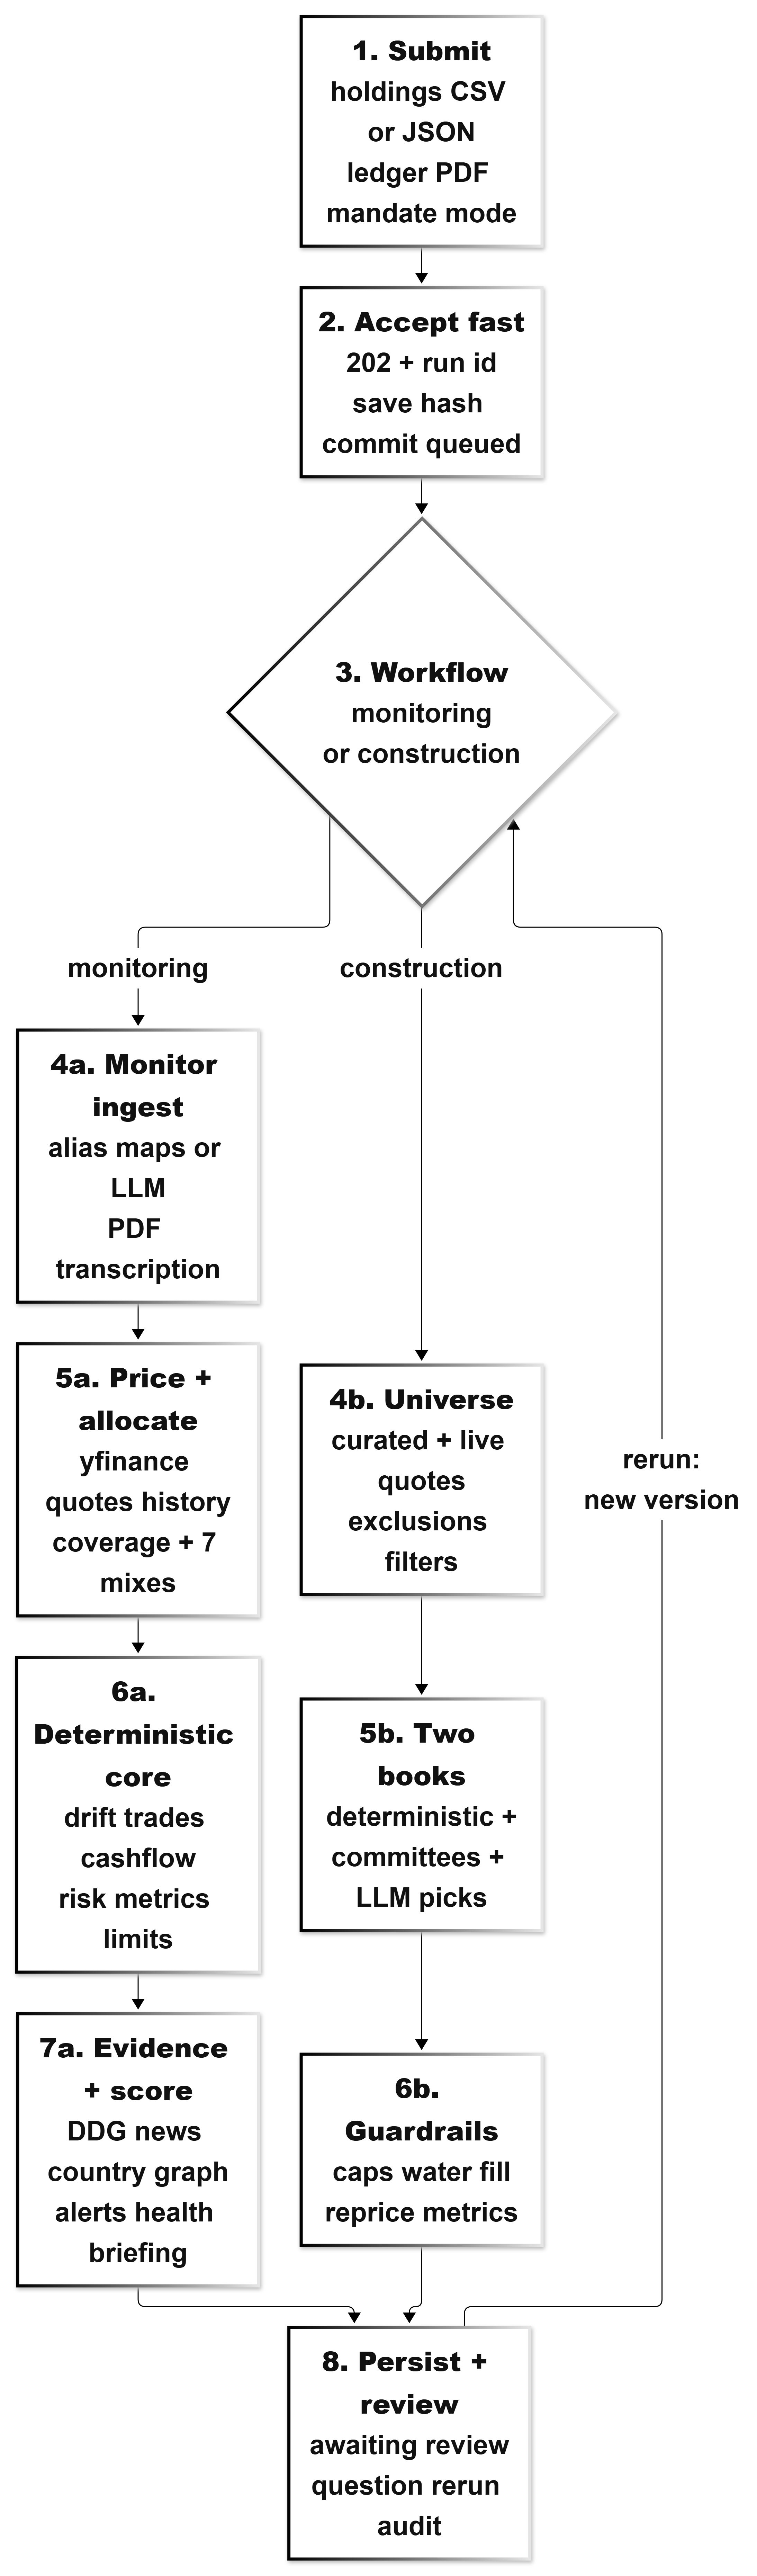
\includegraphics[width=\textwidth,height=0.85\textheight,keepaspectratio]{../diagrams/investment_research/01_flowchart_end-to-end-pipeline-diagram.png}
\caption{End-to-End Pipeline Diagram}
\label{fig:ch06_investment_research-01-flowchart-end-to-end-pipeline-diagram}
\end{figure}

\speaker{Interviewer}{Why do both deterministic and LLM construction books pass through the same guardrails?}

\speaker{Candidate}{To make the decision boundary independent of how a position was selected. An LLM may produce a reasonable idea but violate single-name, sector, exclusion, or minimum-position rules. Shared guardrails ensure every final book satisfies the same policy.}


\speaker{Interviewer}{Now list the main monitoring, construction, and shared components in one place.}

\subsection{Main Components}

\subsubsection{Monitoring Components}

\begin{itemize}[leftmargin=\speakwid]
\item Ingestion and alias normalization.
\item PDF statement transcription.
\item Market-data retrieval and caching.
\item Pricing and allocation.
\item Drift and trade planning.
\item Cash-flow analysis.
\item Risk and limit checks.
\item News scan and country research.
\item Alerts and health scoring.
\item Deterministic and LLM briefings.
\end{itemize}
\subsubsection{Construction Components}

\begin{itemize}[leftmargin=\speakwid]
\item Country research.
\item Universe builder.
\item Committee scoring.
\item Deterministic constructor.
\item LLM advisor.
\item Guardrails and repricing.
\item Feasibility and comparison.
\item Position annotation.
\end{itemize}
\subsubsection{Shared Infrastructure}

\begin{itemize}[leftmargin=\speakwid]
\item FastAPI routes.
\item BackgroundTasks or Celery dispatch.
\item Redis status tracking.
\item Postgres persistence.
\item S3 or ADLS document storage.
\item Review, rerun, Q\&A, and audit APIs.
\end{itemize}

\speaker{Candidate}{Both pipelines share guardrails. Can we now stress-test the key decisions --- holdings, drift, cash flows, and risk?}

\medskip\hrule\medskip
\section{Deep Discussion on Pipeline Decisions}
\label{sec:ch06_investment_research-5-deep-discussion-on-pipeline-decisions}


\speaker{Interviewer}{Let us start with fast accept and background execution --- why not block on upload?}

\subsection{Fast Accept and Background Execution}

\speaker{Interviewer}{Why not complete the analysis inside the upload request?}

\speaker{Candidate}{A run may fetch market history for many holdings, perform multiple news searches, run country research, and make several LLM calls. Holding the HTTP connection open creates timeout risk. The API should save the files, create the run and document rows, set the initial phase, dispatch the job, and return a 202 response with the run ID.}

\speaker{Interviewer}{What are the two execution modes?}

\speaker{Candidate}{When \texttt{USE\_CELERY=0}, the API uses an in-process \texttt{BackgroundTasks} job. When \texttt{USE\_CELERY=1}, it dispatches a Celery task to a worker. Both modes call the same monitoring or construction execution logic.}

\speaker{Interviewer}{Why support both?}

\speaker{Candidate}{BackgroundTasks is easy for local development and a small deployment. Celery provides a more durable and scalable worker model. Supporting both gives a straightforward development path without forcing Celery into every local run.}

\speaker{Interviewer}{What does Redis do?}

\speaker{Candidate}{Redis DB 0 stores live phase information such as queued, ingesting holdings, persisting results, done, or failed. Redis DB 1 acts as the Celery broker and result backend when Celery is enabled. The status tracker is fail-soft; the database remains the terminal source of truth.}

\speaker{Candidate}{That covers the two databases. Can I state the timeouts and retry bounds advisors feel as poll latency?}

\speaker{Interviewer}{Yes.}

\speaker{Candidate}{Live phases in Redis DB 0 carry a 3600-second TTL and never raise into the job, while Celery tasks on DB 1 use JSON serialization, UTC, late acknowledgment, prefetch of one, and two retries spaced at 30 seconds. Uploads persist under S3 or ADLS batch prefixes with filename, content hash, and document type recorded in Postgres, and monitoring persists one commit of holdings, alerts, trades, and briefing rows plus the full raw result, latency, LLM count, health score, and step reasoning before marking the phase done. That is why polling reads Redis first but Postgres decides terminal state.}

\speaker{Interviewer}{What if Redis is unavailable?}

\speaker{Candidate}{The run should still use Postgres status on terminal reads, and the phase update should not crash the job. The tracker latches an unavailable state after a failed ping, which is a recovery limitation.}


\speaker{Interviewer}{How do you ingest messy holdings CSVs and transaction ledgers?}

\subsection{Holdings Ingestion}

\speaker{Interviewer}{How do you normalize arbitrary CSV and JSON holdings?}

\speaker{Candidate}{The ingestion layer maps common aliases to a canonical schema. Symbols are uppercased, quantity defaults to zero when absent, and optional fields are normalized. JSON may be a list or an object containing \texttt{holdings}.}

\speaker{Interviewer}{What if the file has an invalid row?}

\speaker{Candidate}{The loader should skip or report the invalid row according to the parser behavior, but it must not silently create a position with an invented symbol. A production version should return row-level diagnostics to the UI.}

\speaker{Interviewer}{What if a holdings file and a PDF statement are both supplied?}

\speaker{Candidate}{The structured holdings file should be the primary source. The PDF is a fallback when structured holdings are unavailable. The system should not silently merge duplicate positions from both sources unless an explicit reconciliation policy exists.}


\speaker{Candidate}{Ingestion is robust. How should the PDF statement fallback handle holdings transcription?}

\subsection{PDF Statement Transcription}

\speaker{Interviewer}{How does the PDF path work?}

\speaker{Candidate}{My design reads the first twelve pages with PyMuPDF and concatenates page text with page markers. One LLM call returns a holdings array. The prompt requires verbatim transcription of symbol, quantity, price, market value, and cost basis, without calculating or rescaling values.}

\speaker{Interviewer}{What if the statement is scanned?}

\speaker{Candidate}{My design provides no OCR, so the PDF path can fail. I would surface a clear validation error rather than treat an empty extraction as a zero-holding portfolio.}

\speaker{Candidate}{Can we go one level deeper on transcription correctness, since a wrong quantity flows straight into priced market value and drift trades?}

\speaker{Interviewer}{Yes. How do you validate the transcribed holdings beyond JSON schema?}

\speaker{Candidate}{Schema only proves the shape. A correctness gate in \texttt{llm\_validation.py} scores whether each holding is actually grounded: the symbol must appear in the statement text, quantity must be positive, and when quantity, price, and market value are all present, quantity times price must agree with market value within five percent. An empty extraction scores zero, so a scanned or unreadable statement cannot pass as an empty portfolio.}

\speakcont{If confidence is below 0.50, the failed checks are appended to the prompt and the transcription LLM is reinvoked once with a bounded retry. For the advisor this matters because holdings ingestion feeds pricing, drift, and rebalance sizing --- catching a misread quantity at ingest is far cheaper than explaining a phantom breach in the briefing.}


\speaker{Interviewer}{Explain the pricing priority --- how does each holding get its market value?}

\subsection{Pricing Source Priority}

\speaker{Interviewer}{Explain how a holding gets its price.}

\speaker{Candidate}{The deterministic price priority is:}

\begin{enumerate}[leftmargin=\speakwid]
\item Positive price supplied in the holdings file.
\item Live market-data quote.
\item Cost basis divided by quantity, when available.
\item Missing price.
\end{enumerate}
\speakcont{The result records the price source. Missing-price holdings are flagged and excluded from priced market-value calculations, while data coverage shows how much of the portfolio was actually priced.}

\speaker{Interviewer}{Why not let the LLM estimate a price?}

\speaker{Candidate}{A price is decision-bearing numeric data. The LLM may be out of date or hallucinate. It should never be used for valuation or trade sizing.}

\speaker{Interviewer}{What if the portfolio is denominated in USD but a holding is in INR?}

\speaker{Candidate}{The \texttt{base\_currency} is primarily a label; there is no FX conversion in the design. The system should not imply that INR market values have been converted to USD. A production version needs an explicit FX layer before cross-currency aggregation is financially meaningful.}


\speaker{Interviewer}{How do allocation, mandate drift, and breach-only trades work?}

\subsection{Allocation and Mandate Drift}

\speaker{Interviewer}{How do you calculate allocation?}

\speaker{Candidate}{First, price each holding. Then compute total priced market value and aggregate by asset class, sector, region, country, currency, market cap, and individual position. The weight is each bucket's market value divided by the total priced market value.}

\speakcont{For mandate drift, each sleeve has a target and band. The status is within, overweight, underweight, breach over, or breach under. A rebalance trade is created only for a breach. The trade value is:}

\[
\text{trade value} = (\text{target weight} - \text{actual weight}) \times \text{portfolio market value}
\]

\speakcont{Positive means buy and negative means sell.}

\speaker{Interviewer}{Why create trades only for breaches?}

\speaker{Candidate}{Small deviations within the approved band do not justify unnecessary turnover. Breach-only trades reduce noise, transaction costs, and over-trading.}


\speaker{Candidate}{Drift sizing is clear. Shall we reconcile expected versus actual cash flows next?}

\subsection{Cash-Flow Reconciliation}

\speaker{Interviewer}{How do you compare expected and actual income?}

\speaker{Candidate}{Expected income comes from dividend or distribution rate times quantity and the analysis fraction. If the rate is unavailable, the system uses an assumed yield by asset class. Actual cash flow comes from the transactions ledger. The output classifies each holding as on track, missing income, shortfall, excess, or unexpected flow.}

\speaker{Interviewer}{What if there is no ledger?}

\speaker{Candidate}{The system still produces expected income but marks actual income as unavailable and includes a note that no ledger was supplied. It must not call the expected figure actual.}

\speaker{Interviewer}{What about a one-time large withdrawal?}

\speaker{Candidate}{The cash-flow logic identifies non-held income, fees, withdrawals, and taxes. Large unexpected flows cross a configured absolute threshold and generate alerts.}


\speaker{Interviewer}{Which risk metrics and limit checks do you compute on priced holdings?}

\subsection{Risk Metrics and Limits}

\speaker{Interviewer}{Which risk metrics do you calculate?}

\speaker{Candidate}{Depending on available history, the system calculates volatility, annualized return, maximum drawdown, VaR at 95 percent, beta, tracking error, HHI, effective number of holdings, top-one and top-five concentration, largest position, and dividend yield.}

\speakcont{Risk limits include single-name concentration, sector concentration, volatility ceiling, drawdown alert, VaR, tracking error, and minimum cash when configured.}

\speaker{Interviewer}{What happens when there is not enough history?}

\speaker{Candidate}{The metric becomes unavailable rather than being fabricated. The result records data coverage and missing-history limitations. Limit checks for unavailable metrics should be marked not available rather than breached.}


\speaker{Candidate}{Risk math is covered. How do news signals and country research enrich the review?}

\subsection{News and Country Research}

\speaker{Interviewer}{Why include news if the portfolio score is deterministic?}

\speaker{Candidate}{News can identify emerging risks that are not yet reflected in price or allocation. It is useful context, but it should not override a deterministic limit or create an unbounded score. High news severity is capped at medium in downstream alerts and scoring.}

\speaker{Interviewer}{How does the system avoid bad ticker searches?}

\speaker{Candidate}{It maps symbols to company names and passes names to the query builder. Exchange suffixes such as \texttt{.NS} or \texttt{.L} are stripped where necessary because raw tickers often produce poor search results.}

\speaker{Interviewer}{What if news classification fails?}

\speaker{Candidate}{The system uses keyword fallback. It can identify terms such as lawsuit, probe, downgrade, or regulatory action and produce a bounded risk scan. If collection fails entirely, the run continues with a data-gap note.}

\speaker{Candidate}{Before country research, can we pin down how news classification is validated, since it becomes advisor-facing emerging-risk alerts?}

\speaker{Interviewer}{Yes. What does the classification gate check?}

\speaker{Candidate}{The gate in \texttt{osint/scan.py} calls \texttt{score\_classification} on every proposed finding: the category must belong to the eight allowed risk dimensions, severity must be low, medium, or high, and the summary must be grounded in the collected snippets rather than invented. An empty benign scan scores 0.55 because no findings can still be correct, while a scan with off-vocabulary categories or ungrounded summaries scores below 0.50.}

\speakcont{On failure the validator lists each failed finding, appends that list to the synthesis prompt, and reinvokes the classifier once. If the retry still fails, the keyword fallback applies and downstream alerts and health scoring still cap news severity at medium, so a loud headline can never flip a portfolio to critical when deterministic limits are clean.}

\speaker{Interviewer}{What is country research used for?}

\speaker{Candidate}{The country research pipeline creates profiles for the top held countries. It uses a real LangGraph StateGraph with multiple research nodes. Findings become portfolio context and may create capped emerging-risk or country alerts.}


\speaker{Interviewer}{How does the health score combine drift, concentration, and risk into one band?}

\subsection{Health Score}

\speaker{Interviewer}{How is the portfolio health score different from raw risk metrics?}

\speaker{Candidate}{Raw metrics describe individual properties such as volatility or drawdown. The health score combines eight factor families: drift, concentration, volatility, drawdown, cash flow, limit breaches, emerging risk, and country risk. Each factor has a weight and severity multiplier. The normalized score maps to healthy, watch, elevated, or critical.}

\speaker{Interviewer}{Why not ask the LLM to assign the health band?}

\speaker{Candidate}{Because the band is a policy output. It must be reproducible and explainable. The LLM can write a briefing that explains the score, but Python determines the score and band.}


\speaker{Candidate}{Health scoring is deterministic. Shall we compare the committee lenses --- VLRT, VCST, and peers?}

\subsection{Investment Committees}

\speaker{Interviewer}{Explain the committee frameworks.}

\speaker{Candidate}{The construction workflow can select one or more research lenses:}

\begin{itemize}[leftmargin=\speakwid]
\item VLRT: valuation, liquidity, risk appetite, and timing.
\item VCST: valuation, cycle, sentiment, and trigger.
\item SQL: size, quality, and longevity.
\item OPCO-FINCO: operating company, financial company, business, and value.
\item BMV: business, management, and valuation with sequential gates.
\end{itemize}
\speakcont{The committee legs calculate deterministic scores. LLMs may write one-line commentary. The combined scores and reasons are attached to selected positions for auditability.}

\speaker{Candidate}{The lens names are clear. Can I record how each lens scores, since construction reasons cite these legs?}

\speaker{Interviewer}{Keep it concise.}

\speaker{Candidate}{VLRT blends valuation 30, liquidity 25, risk appetite 25, and timing 20, with valuation rewarding low price-to-earnings and high yield and liquidity rewarding large caps and fund vehicles. VCST uses valuation 30, cycle 25, sentiment 25, and trigger 20, where sentiment comes from bounded company and sector searches and adverse triggers pull the leg down. SQL multiplies business stability by management execution for quality with 40 percent weight alongside size 25 and longevity 35. OPCO-FINCO weights operating company 20, financial company 15, business 35, and value 30. BMV is a sequential gate: business 40, then management 35, then valuation 25, where a business score below 0.35 drops the name to 0.30 and a management score below 0.35 drops it to 0.40 regardless of later legs. Every committee returns a zero-to-one combined score plus a fail-soft one-line view, and those scores travel on each selected position for the audit trail.}

\speaker{Interviewer}{Why use multiple committees?}

\speaker{Candidate}{Different investment teams evaluate assets through different lenses. The system can compare views while retaining a common deterministic universe, score range, and guardrail layer.}


\speaker{Interviewer}{How does the deterministic book build sleeve targets into capped positions?}

\subsection{Deterministic Construction}

\speaker{Interviewer}{How does the deterministic book get built?}

\speaker{Candidate}{The constructor applies sleeve targets, selects sector-diverse candidates, caps the number of names per sleeve and sector, and assigns within-sleeve weights using equal weight, return tilt, inverse volatility, or risk parity. It then applies guardrails and computes amounts and shares.}

\speaker{Candidate}{Sizing rules are clear. Can I detail the universe filters and the feasibility verdicts, since they decide which names the LLM advisor even sees?}

\speaker{Interviewer}{Yes.}

\speaker{Candidate}{The universe starts from explicit symbols or curated country sleeves for the United States, United Kingdom, Japan, Germany, and India, with theme baskets such as clean energy, AI, semiconductors, cyber, water, and gold matched by substring, plus granular fund categories and seed pools like broad equity, aggregate bond, bills, and gold tickers. Filters remove exclusions, enforce minimum dividend, maximum price-to-earnings, maximum expense, instrument and region preferences, and a country credit floor that excludes stressed countries with two or more high findings while subtracting a penalty of 0, 1.5, or 3 percent from expected returns. Deterministic selection caps at eight names per sleeve and two per sector with a diverse first pass and return-fill second pass.}

\speakcont{Feasibility then converts the request into an implied annual target, treating values above one as percent and deriving value targets from investable amount and horizon, and classifies it as no-target, achievable, ambitious when above expected plus five percent, or unrealistic above 50 percent or the universe ceiling. The deterministic-versus-LLM comparison reports Jaccard overlap, sleeve and metric deltas, guardrail correction counts, and a note when the largest sleeve differs by two percent or more, so the advisor sees divergence in numbers rather than narrative.}

\speaker{Interviewer}{How does it avoid over-concentration?}

\speaker{Candidate}{It applies single-name and sector caps through a water-fill redistribution process. Weight above a cap is redistributed among under-cap positions. The algorithm iterates with bounded loops and records corrections or residual cash when constraints are infeasible.}


\speaker{Candidate}{Deterministic sizing is clear. What exactly may the LLM advisor propose --- and what gets whitelisted?}

\subsection{LLM Construction}

\speaker{Interviewer}{What exactly does the LLM constructor receive?}

\speaker{Candidate}{It receives a candidate digest containing only approved universe symbols, market metadata, expected returns, volatility, news risk, and committee scores. The prompt asks it to propose weights, reasons, and committee-specific rationale.}

\speakcont{After the response:}

\begin{enumerate}[leftmargin=\speakwid]
\item Unknown symbols are dropped.
\item Non-positive weights are dropped.
\item The portfolio is sent through shared guardrails.
\item Prices and shares are recomputed deterministically.
\item Expected metrics are recalculated.
\end{enumerate}
\speaker{Interviewer}{Why not trust the weights returned by the LLM?}

\speaker{Candidate}{Because the model may violate constraints or produce arithmetic inconsistencies. The LLM output is an idea proposal, not the final numeric result.}

\speaker{Candidate}{The whitelist is schema-level. Can I spell out the numeric correctness gate on the LLM book, since it guards the proposed weights advisors see?}

\speaker{Interviewer}{Please do. What fails the construction gate?}

\speaker{Candidate}{The \texttt{score\_suggestion} check requires every pick to use a universe ticker, so a hallucinated symbol fails hard, each weight to lie in zero to cap with a default cap of 0.35 unless the mandate sets a tighter single-name cap, weights to sum to approximately one, and each reason to be non-empty. An empty pick list scores zero. Below 0.50 confidence the failed validations are appended to the advisor prompt and the LLM is reinvoked through the shared \texttt{validate\_with\_retry} helper, still bounded and fail-soft.}

\speakcont{Only survivors reach \texttt{guardrails.enforce} and \texttt{finalise\_positions}, where amounts, shares, invested value, and cash residual are recomputed in Python. That is why a plausible-sounding LLM weight can never silently become a trade: it must first survive whitelist, numeric, and guardrail gates.}


\speaker{Interviewer}{Finally, how do briefings, Q\&A, and review stay grounded in computed results?}

\subsection{Briefing, Q\&A, and Review}

\speaker{Interviewer}{How is the briefing generated?}

\speaker{Candidate}{A deterministic briefing is always built from the computed result. If the mode is \texttt{llm} or \texttt{both} and the gateway is available, an LLM briefing receives a compact authoritative snapshot. The prompt says not to recompute or change figures. If it fails, the deterministic briefing remains available.}

\speakcont{Q\&A also receives only the compact result and the user's question. It must admit when the answer is not present.}

\speakcont{Review actions are stored through the review endpoint. Approval and rejection change the run status. Corrected fields are recorded but do not automatically recalculate the result.}


\speaker{Candidate}{Pipeline trade-offs are clear. Shall we pin down exactly which numbers deterministic Python owns?}

\medskip\hrule\medskip
\section{Deterministic Portfolio Analytics Core}
\label{sec:ch06_investment_research-6-deterministic-portfolio-analytics-core}

\speaker{Interviewer}{Now go deeper into the calculations. I want to understand what Python owns.}

\subsection{Pricing and Market Value}

For each holding, the system chooses a price from the configured priority order. It calculates market value and price coverage. Holdings without usable prices remain visible but are excluded from priced allocation totals.


\speaker{Interviewer}{Holdings are priced. How do you aggregate allocation across sleeves and sectors?}

\subsection{Allocation}

For a bucket such as asset class or sector:

\[
\text{weight}_b = \frac{\text{market value}_b}{\text{total priced market value}}
\]

The result stores allocation by asset class, sector, region, country, currency, market cap, and position.


\speaker{Candidate}{Allocation is clear. Which return, volatility, and drawdown primitives feed risk next?}

\subsection{Analytics Primitives}

The deterministic analytics module calculates:

\begin{itemize}[leftmargin=\speakwid]
\item Daily returns.
\item Annualized volatility.
\item Annualized return.
\item Maximum drawdown.
\item VaR at the 95 percent level.
\item Beta.
\item Tracking error.
\item Herfindahl-Hirschman Index.
\item Effective number of holdings.
\item Portfolio return series.
\end{itemize}
Short or missing history produces null or unavailable metrics.


\speaker{Interviewer}{How do mandate bands turn into breach-only rebalance trades?}

\subsection{Drift and Rebalancing}

Mandate targets have tolerance bands. A sleeve breaches when its actual weight exceeds the upper or lower band. The rebalancing plan contains only breach trades, with buy or sell action, signed trade value, turnover, transaction-cost estimate, and rationale.


\speaker{Candidate}{Trades are sized. How do expected and ledger cash flows reconcile?}

\subsection{Cash Flow}

Expected cash flow is calculated from known distributions or assumed asset-class yields. Actual cash flow comes from the ledger. Variance, tolerance, materiality floor, unexpected flows, and severity are deterministic policy rules.

\speaker{Candidate}{Those rules are policy, not heuristics. Shall I state the exact thresholds so reconciliation is reproducible?}

\speaker{Interviewer}{Yes. What are they?}

\speaker{Candidate}{Expected income uses dividend rate times quantity times the analysis fraction, falling back to assumed yields of 1.5 percent equity, 4 percent fixed income, 5 percent cash, 3 percent alternatives, 3.5 percent real estate, 2 percent multi-asset, and zero for commodity and other. Variances within 10 percent are on track, tiny expected values under 250 with no actual are skipped by the materiality floor, and non-held fees, withdrawals, and taxes above an absolute 10000 become unexpected flows, rising to high severity at 50000. For an advisor this means a missing ledger reads as unavailable rather than a false shortfall, while a genuine large withdrawal still escalates to an alert.}


\speaker{Interviewer}{Which concentration, volatility, and drawdown limits gate the portfolio?}

\subsection{Risk Limits}

Risk limits evaluate single-name weight, sector weight, volatility, drawdown, VaR, tracking error, and cash. A limit can be breached, near its limit, within limit, or unavailable.

\speaker{Candidate}{Can I pin down the mandate numbers behind those limits, since drift and ceiling breaches drive the rebalance trades?}

\speaker{Interviewer}{Go ahead.}

\speaker{Candidate}{Sleeve targets are conservative 30 equity, 55 fixed income, 10 cash, 5 alternatives; balanced 55, 35, 5, 5; growth 75, 18, 2, 5; aggressive 90, 5, 0, 5, with bands of 5, 5, 6, and 7 points and benchmarks AOK, AOM, AOR, and AOA. Volatility ceilings are 10, 14, 18, and 24 percent by mandate. Single-name breaches at 10 percent, sector at 30 percent with Unclassified exempt, drawdown alert at 20 percent, VaR at 4 percent, tracking error at 10 percent, and anything at or above 90 percent of a limit warns at medium before it breaches at high. Missing history yields not-available rather than a fabricated pass.}


\speaker{Candidate}{Limits are set. How do drift, risk, and news findings become sorted alerts?}

\subsection{Alerts}

Alerts are built from:

\begin{enumerate}[leftmargin=\speakwid]
\item Rebalance breaches.
\item Single-name concentration.
\item Sector concentration.
\item Risk-limit breaches or warnings.
\item Cash-flow anomalies.
\item Unpriced holdings.
\item Emerging news risk.
\item Country research findings.
\end{enumerate}
They are sorted by severity and contain title, detail, evidence, recommended action, and symbols.


\speaker{Interviewer}{How do those alerts roll up into a single health score and band?}

\subsection{Health Score}

The score combines weighted factor contributions:

\[
\text{raw score} = \sum_i \text{factor weight}_i \times \text{severity multiplier}_i
\]

\[
\text{normalized score} = \min(100, \text{raw score})
\]

The band maps to healthy, watch, elevated, or critical. News and country signals are intentionally capped so that contextual research cannot dominate hard portfolio constraints.

\speaker{Candidate}{Score bands are set. Can I record the exact factor weights and guardrail loop bounds, since they decide the band advisors brief to clients?}

\speaker{Interviewer}{Yes, briefly.}

\speaker{Candidate}{Health uses weights of drift 20, concentration 18, volatility 18, drawdown 16, cash flow 10, limit breach 22, emerging 12, and country 10, with severity multipliers of zero for low, 0.6 for medium, 1 for high, and 1.5 for critical, normalized at 100 and banded at 25, 50, and 75. Guardrails then enforce exclusions, normalization, minimum position, and a 50-iteration alternate projection between single-name water-fill with 200 inner iterations and sector proportional scale-down, recording every fix as a correction and spilling infeasible residuals to cash. That pairing is why the same breach that lowers the health band also produces a capped, repriced trade proposal rather than free prose.}


\speaker{Candidate}{Scoring is reproducible. Which guardrails cap the constructed books?}

\subsection{Construction Guardrails}

Guardrails enforce:

\begin{itemize}[leftmargin=\speakwid]
\item Exclusions.
\item Single-name cap.
\item Sector cap.
\item Minimum position.
\item Weight normalization.
\item Residual cash handling.
\item Maximum holdings and universe constraints.
\end{itemize}
After guardrails, Python recomputes amount, shares, invested value, cash residual, and expected metrics. No LLM numeric output is authoritative.


\speaker{Interviewer}{Show me the deterministic analytics flow end to end.}

\subsection{Deterministic Analytics Flow}

\begin{figure}[htbp]
\centering
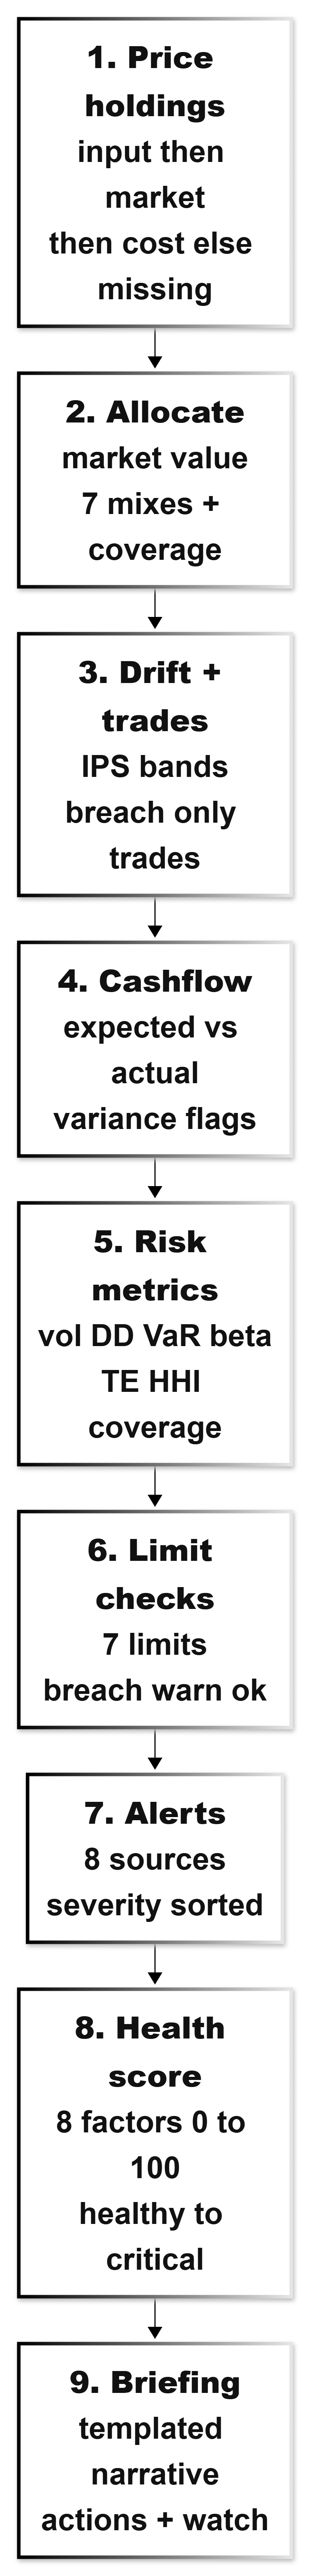
\includegraphics[width=\textwidth,height=0.85\textheight,keepaspectratio]{../diagrams/investment_research/02_flowchart_deterministic-analytics-flow.png}
\caption{Deterministic Analytics Flow}
\label{fig:ch06_investment_research-02-flowchart-deterministic-analytics-flow}
\end{figure}


\speaker{Candidate}{The math is pinned down. Can we discuss how briefings and Q\&A explain drift and risk without rewriting numbers?}

\medskip\hrule\medskip
\section{Memo Generation and Q\&A}
\label{sec:ch06_investment_research-7-memo-generation-and-q-a}

\speaker{Interviewer}{Explain how the system creates an understandable research output.}

\speaker{Candidate}{The system creates a deterministic briefing first. It covers the portfolio health score, allocation, risk, cash flow, recommended actions, and watch items.}

\speakcont{If enabled, an LLM receives compact JSON containing:}

\begin{itemize}[leftmargin=\speakwid]
\item Portfolio name and mandate.
\item Market value.
\item Health band and score.
\item Asset-class mix.
\item Drift breaches.
\item Rebalance summary.
\item Risk metrics.
\item Limit breaches.
\item Cash-flow summary.
\item Alerts.
\item Emerging-risk context.
\end{itemize}
\speakcont{The LLM writes executive, allocation, risk, cash-flow, action, and watch-item sections. It is instructed to treat the supplied snapshot as authoritative.}

\speaker{Interviewer}{What if the LLM says volatility is 12 percent when the computed value is 14 percent?}

\speaker{Candidate}{The system should treat the computed value as authoritative. A production hardening step should validate narrative numbers against the snapshot or use a string-only narrative schema that avoids free numeric restatement. The design relies primarily on the prompt and should add post-generation grounding checks.}

\speaker{Interviewer}{How does Q\&A work?}

\speaker{Candidate}{The question endpoint sends the user question and a compact portfolio snapshot to the LLM. The answer must use only supplied figures, admit missing information, and avoid inventing trades, alerts, or metrics.}

\speaker{Interviewer}{Can Q\&A place a trade?}

\speaker{Candidate}{No. It only explains the stored analysis. Trade execution is outside the system.}


\speaker{Candidate}{Briefings stay grounded. Shall I now give the full architecture --- API, Postgres, Redis, and the UI review flow?}

\medskip\hrule\medskip
\section{High-Level Design}
\label{sec:ch06_investment_research-8-high-level-design}

\speaker{Interviewer}{Give me the full architecture in one view.}

\speaker{Candidate}{The architecture contains a fast API layer, durable database state, optional Redis and Celery execution, deterministic analytics services, optional research enrichment, and a UI for review.}

\subsection{Architecture Components}

\begin{enumerate}[leftmargin=\speakwid]
\item Vanilla JavaScript production UI.
\item Optional Streamlit development UI.
\item FastAPI routes under \texttt{/portfolios}.
\item Postgres with \texttt{portfolio\_runs} and child result tables.
\item S3 or ADLS upload storage.
\item Redis DB 0 for live phases.
\item Redis DB 1 for Celery when enabled.
\item BackgroundTasks or Celery worker.
\item yfinance market-data integration.
\item DuckDuckGo news integration.
\item Real LangGraph country-research workflow.
\item Deterministic monitoring and construction modules.
\item Optional LLM gateway.
\item Review, rerun, Q\&A, and audit endpoints.
\end{enumerate}

\speaker{Interviewer}{Show me that architecture in one diagram.}

\subsection{High-Level Architecture Diagram}

\begin{figure}[htbp]
\centering
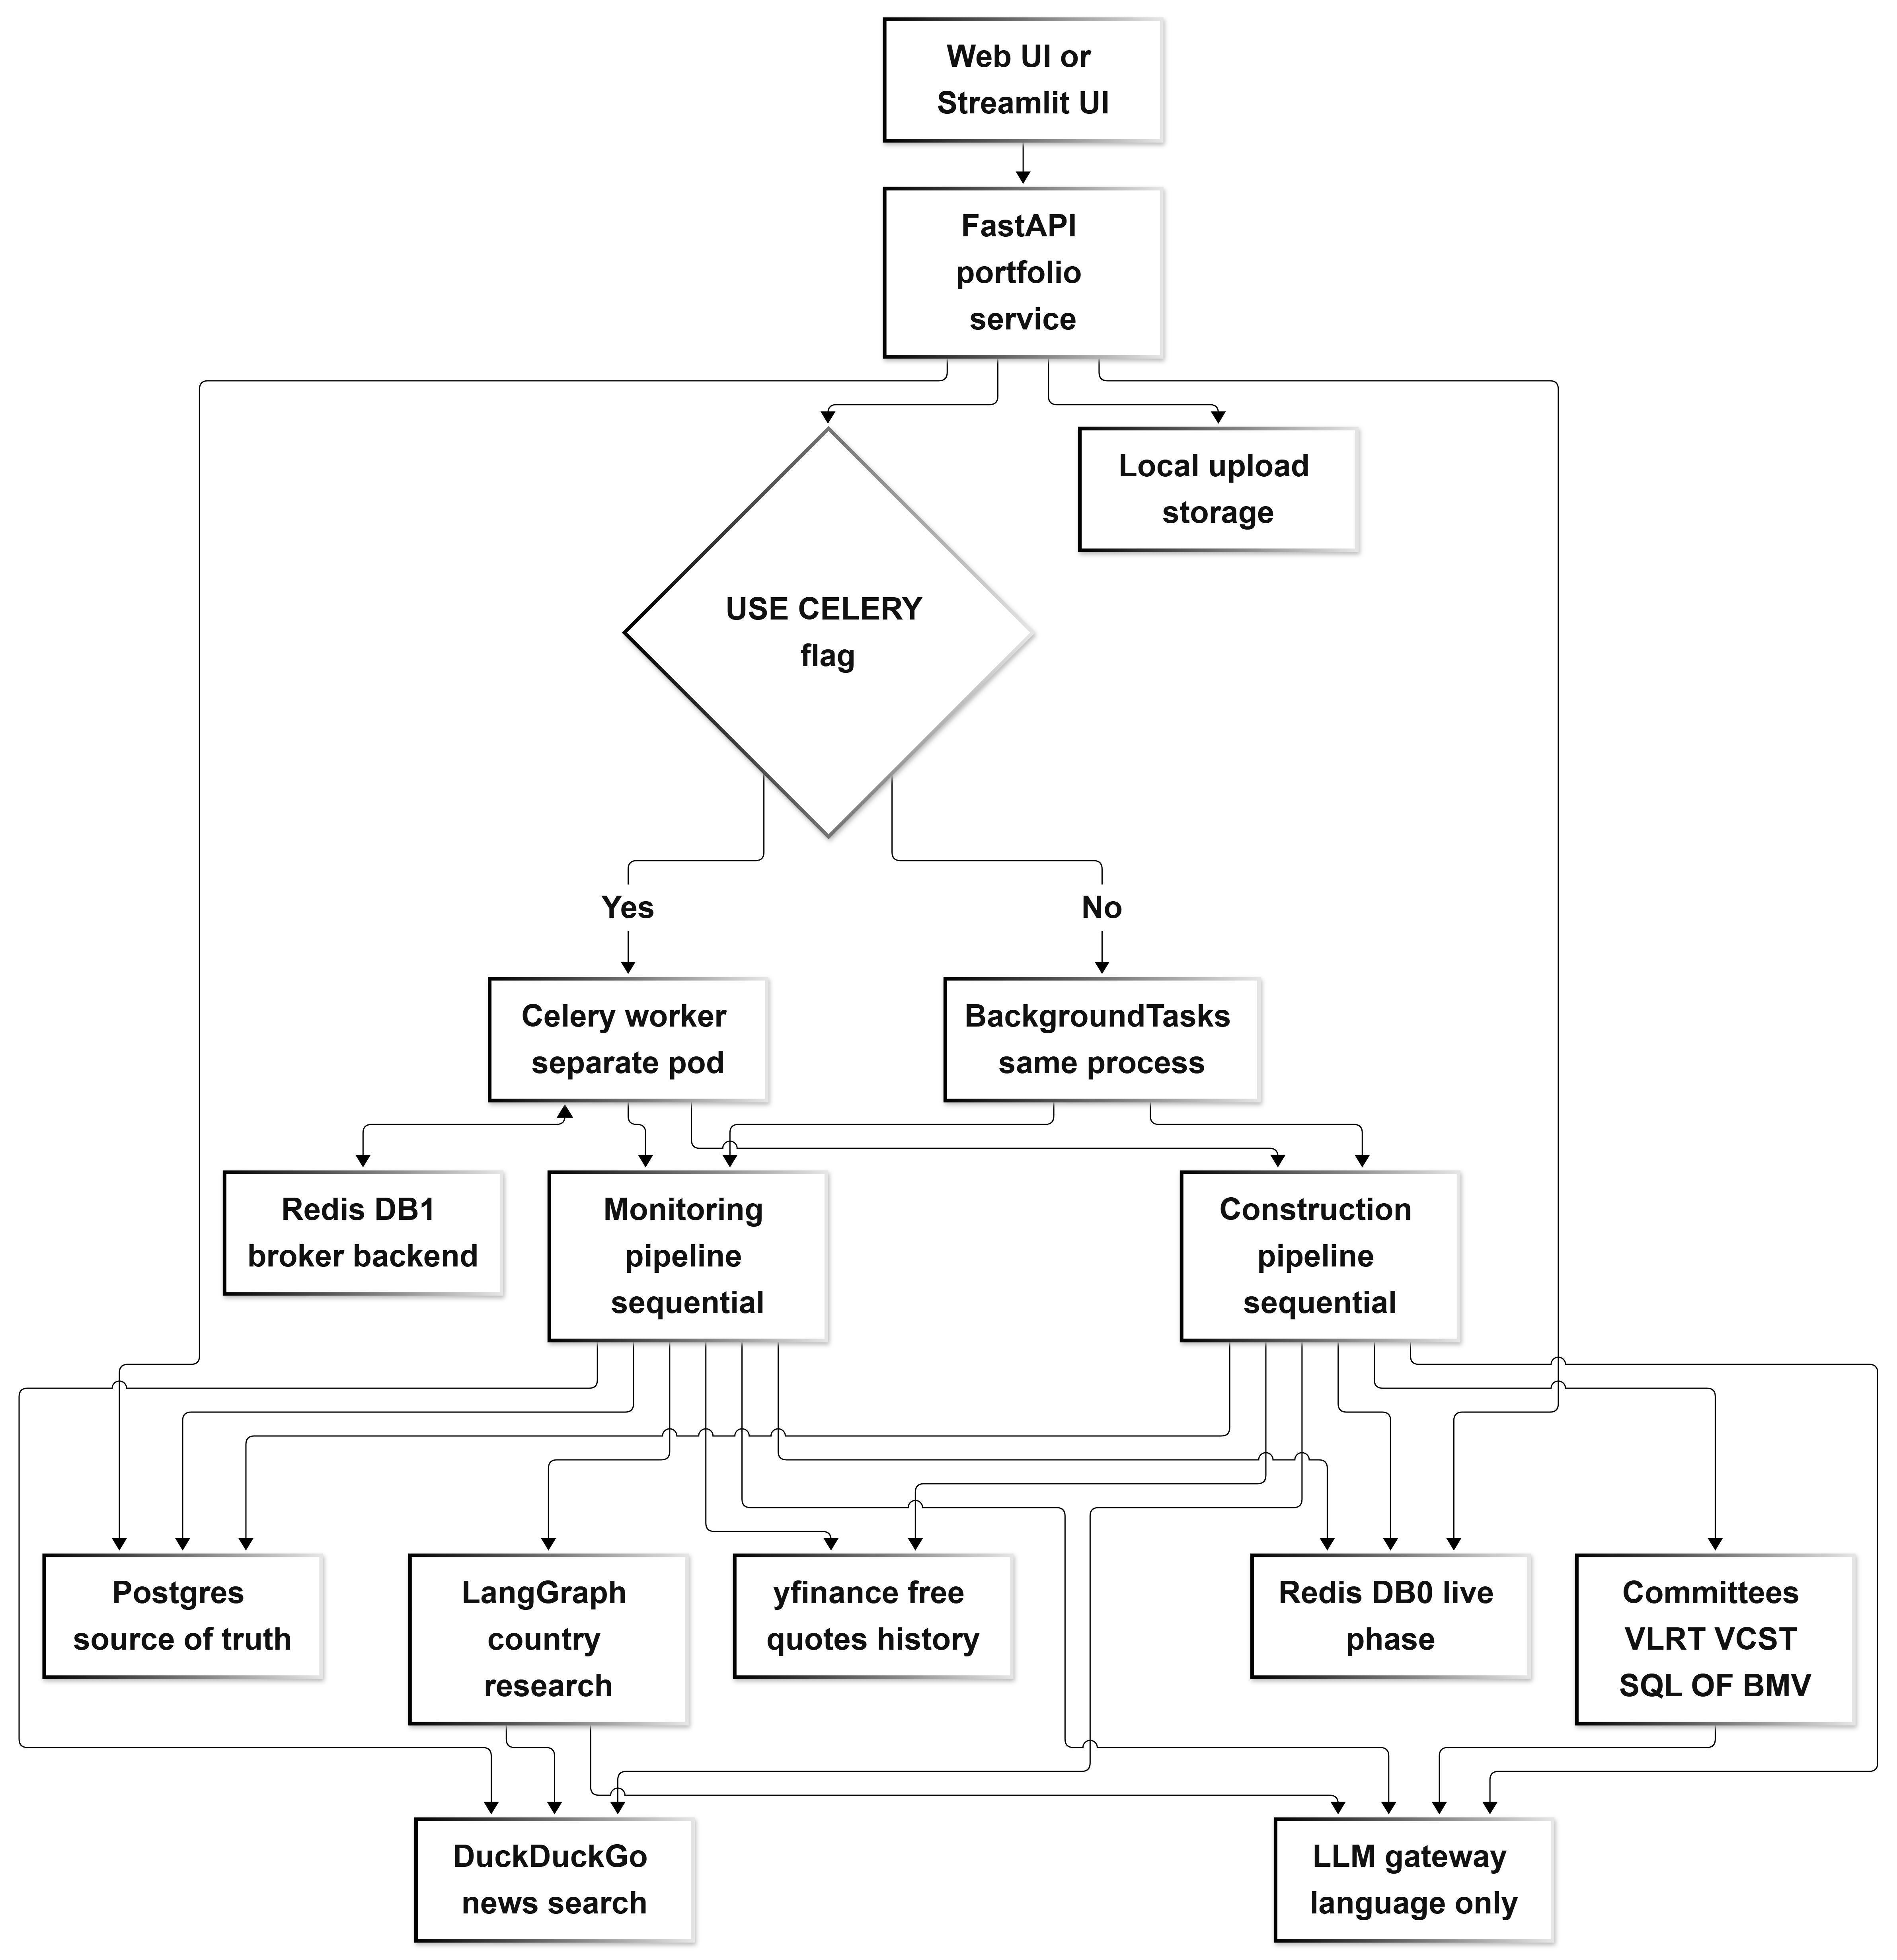
\includegraphics[width=\textwidth,height=0.85\textheight,keepaspectratio]{../diagrams/investment_research/03_flowchart_high-level-architecture-diagram.png}
\caption{High-Level Architecture Diagram}
\label{fig:ch06_investment_research-03-flowchart-high-level-architecture-diagram}
\end{figure}

\speaker{Interviewer}{Why is \texttt{agent\_graph.py} not necessarily a LangGraph workflow?}

\speaker{Candidate}{The name is historical. Monitoring and construction orchestration are sequential Python functions. The real LangGraph workflow is country research in \texttt{research/graph.py}. I would not claim agentic graph behavior where the design does not provide it.}


\speaker{Interviewer}{Now take me through the low-level design --- request lifecycles, core modules, and failure handling.}

\medskip\hrule\medskip
\section{Low-Level Design}
\label{sec:ch06_investment_research-9-low-level-design}

\speaker{Interviewer}{Now go into low-level design. Explain the request lifecycle and modules.}

\subsection{Monitoring Request Lifecycle}

\begin{itemize}[leftmargin=\speakwid]
\item \texttt{POST /portfolios} accepts multipart form data.
\item Files are saved and hashed.
\item A \texttt{portfolio\_runs} row is inserted with status \texttt{created}.
\item \texttt{portfolio\_documents} rows are inserted.
\item The transaction commits.
\item Redis phase becomes \texttt{queued}.
\item The job is dispatched to BackgroundTasks or Celery.
\item The worker marks the run \texttt{processing}.
\item Monitoring modules execute in order.
\item Holdings, alerts, trades, and briefing rows are persisted.
\item The run becomes \texttt{awaiting\_review}.
\end{itemize}

\speaker{Candidate}{Monitoring lifecycle is clear. Shall I trace the construction request lifecycle next?}

\subsection{Construction Request Lifecycle}

\begin{itemize}[leftmargin=\speakwid]
\item \texttt{POST /portfolios/construct} accepts JSON or multipart-equivalent input.
\item A construction run is created with \texttt{result\_type=construction}.
\item The job builds research and universe data.
\item Deterministic and optional LLM books are created.
\item Shared guardrails are applied.
\item Positions and comparison metrics are computed.
\item The result is persisted using the same run and child tables.
\end{itemize}

\speaker{Interviewer}{Which modules own ingestion, drift, risk, guardrails, and research?}

\subsection{Core Modules}

\begin{itemize}[leftmargin=\speakwid]
\item \texttt{ingest.py} for holdings and transaction normalization.
\item \texttt{statement\_extract.py} for PDF transcription.
\item \texttt{marketdata.py} for quotes and history.
\item \texttt{allocation.py} for pricing and breakdowns.
\item \texttt{drift.py} for target comparison and trade plans.
\item \texttt{cashflow.py} for income analysis.
\item \texttt{risk.py} for metrics and limits.
\item \texttt{alerts.py} for severity-sorted alerts.
\item \texttt{scoring.py} for health score.
\item \texttt{universe.py} for construction candidates.
\item \texttt{construct/deterministic.py} for deterministic construction.
\item \texttt{construct/llm\_advisor.py} for optional LLM construction.
\item \texttt{construct/guardrails.py} for shared constraints.
\item \texttt{research/graph.py} for country research.
\item \texttt{osint/scan.py} for news interpretation.
\item \texttt{db/persist.py} for atomic result persistence.
\end{itemize}

\speaker{Candidate}{One module is missing from that list and it owns all three gates we just discussed. Shall I add it?}

\speaker{Interviewer}{Yes. How is the validation layer wired?}

\speaker{Candidate}{The pure-stdlib module \texttt{llm\_validation.py} exposes \texttt{score\_classification}, \texttt{score\_extraction}, and \texttt{score\_suggestion} plus a shared \texttt{validate\_with\_retry} helper with \texttt{CONFIDENCE\_THRESHOLD = 0.50} and \texttt{MAX\_ATTEMPTS = 3}. It is wired into statement extraction with one reinvocation and into news synthesis in \texttt{osint/scan.py} with one reinvocation before keyword fallback, and it is covered by four offline tests in \texttt{tests/test\_llm\_validation.py}.}

\speakcont{The pattern is always the same: score the LLM output against deterministic evidence, list the failures, append them to the prompt, and retry bounded. Briefing prose, Q\&A answers, and pros-and-cons annotations remain prompt-trusted in the design, so they rely on snapshot-grounded prompts and the string-only briefing schema rather than this gate.}

\speaker{Interviewer}{What happens when market data, news, country research, or the LLM gateway fails?}

\subsection{Failure Handling}

\speaker{Interviewer}{What if market data is unavailable for one symbol?}

\speaker{Candidate}{The quote and history calls fail softly. The position may remain unpriced or have missing risk metrics. The result should show lower data coverage and alerts for unpriced holdings rather than silently treating the position as zero.}

\speaker{Interviewer}{What if all market data is unavailable?}

\speaker{Candidate}{The run can still persist holdings and input-derived values, but allocation, risk, and health output should clearly indicate that market data is unavailable. A production policy may route the run to validation review.}

\speaker{Interviewer}{What if news or country research fails?}

\speaker{Candidate}{The run continues with an evidence-gap marker. Contextual research is optional and must not block deterministic monitoring.}

\speaker{Interviewer}{What if the LLM gateway fails in \texttt{mode=llm}?}

\speaker{Candidate}{The system falls back to deterministic briefing. LLM construction falls back to a deterministic portfolio labelled as an LLM-mode fallback. The result should expose that fallback in method and reasoning.}


\speaker{Candidate}{Failures degrade gracefully. Shall we define rerun lineage on the same uploaded documents?}

\subsection{Re-run Behavior}

\speaker{Interviewer}{How does rerun work?}

\speaker{Candidate}{A rerun creates a new \texttt{portfolio\_runs} row with \texttt{parent\_run\_id}, re-links the same uploaded documents, and applies the requested overrides such as mandate, news flag, question, or instruction. The new run gets its own results and audit lineage.}


\speaker{Interviewer}{What happens when a reviewer approves, rejects, or corrects a run?}

\subsection{Review Behavior}

\speaker{Interviewer}{What happens when a reviewer approves or rejects a run?}

\speaker{Candidate}{A review row is inserted. For approved or rejected actions, the run status transitions accordingly. A corrected action records corrected fields and reason, but the design does not automatically regenerate the analytical result.}


\speaker{Candidate}{Review states are stored. Shall we close the loop with the audit trail for holdings, trades, and reviews?}

\subsection{Audit Behavior}

\speaker{Interviewer}{What does the audit endpoint return?}

\speaker{Candidate}{It returns the run identity and parent, model and requester metadata, timestamps, documents, holdings, alerts, and reviews. The full raw result remains available in the portfolio response and database JSON.}

\speaker{Candidate}{Audit trace is covered. Can we lock down the full endpoint contract before the data model, since advisors poll status and then read results?}

\speaker{Interviewer}{Yes. What are the exact endpoints?}

\speaker{Candidate}{Nine routes under one FastAPI service: \texttt{GET /health} returns status ok; \texttt{GET /portfolios} lists run summaries newest first with no pagination; \texttt{POST /portfolios} accepts multipart holdings, transactions, statement, mandate, mode, base currency, names, news flag, question, and requester and returns 202 with a created run; \texttt{POST /portfolios/construct} accepts a construction request as JSON or multipart equivalent; \texttt{GET /portfolios/\{id\}/status} reads the Redis phase first and Postgres on terminal states; \texttt{GET /portfolios/\{id\}} returns the full result with documents, reasoning, latency, and LLM count; \texttt{POST /portfolios/\{id\}/rerun} creates a child run that re-links parent documents; \texttt{POST /portfolios/\{id\}/question} answers from the stored snapshot and returns 409 when no result exists yet; \texttt{POST /portfolios/\{id\}/review} records any action string but only approved or rejected transitions the run; \texttt{GET /portfolios/\{id\}/audit} returns the trace.}

\speakcont{Two behaviors matter operationally: a missing holdings file surfaces as a 500 rather than a 400, and a bogus ID polled against Redis can look like processing because there is no Postgres row check. Both are gaps the API hardening pass should fix, while every successful monitoring or construction job ends in \texttt{awaiting\_review} and failures land in \texttt{validation\_review} with no completion timestamp.}


\speaker{Interviewer}{Walk me through the data model --- runs, holdings, alerts, trades, briefings, and reviews.}

\medskip\hrule\medskip
\section{Data Modeling}
\label{sec:ch06_investment_research-10-data-modeling}

\speaker{Interviewer}{Now describe the data model in detail. Include the entity relationship diagram and tables.}

\speaker{Candidate}{The model is anchored on \texttt{portfolio\_runs}. Every monitoring or construction execution is one run. Child tables store queryable outputs, while \texttt{raw\_result} stores the full serialized monitoring or construction result.}

\subsection{Entity Relationship Diagram}

\begin{figure}[htbp]
\centering
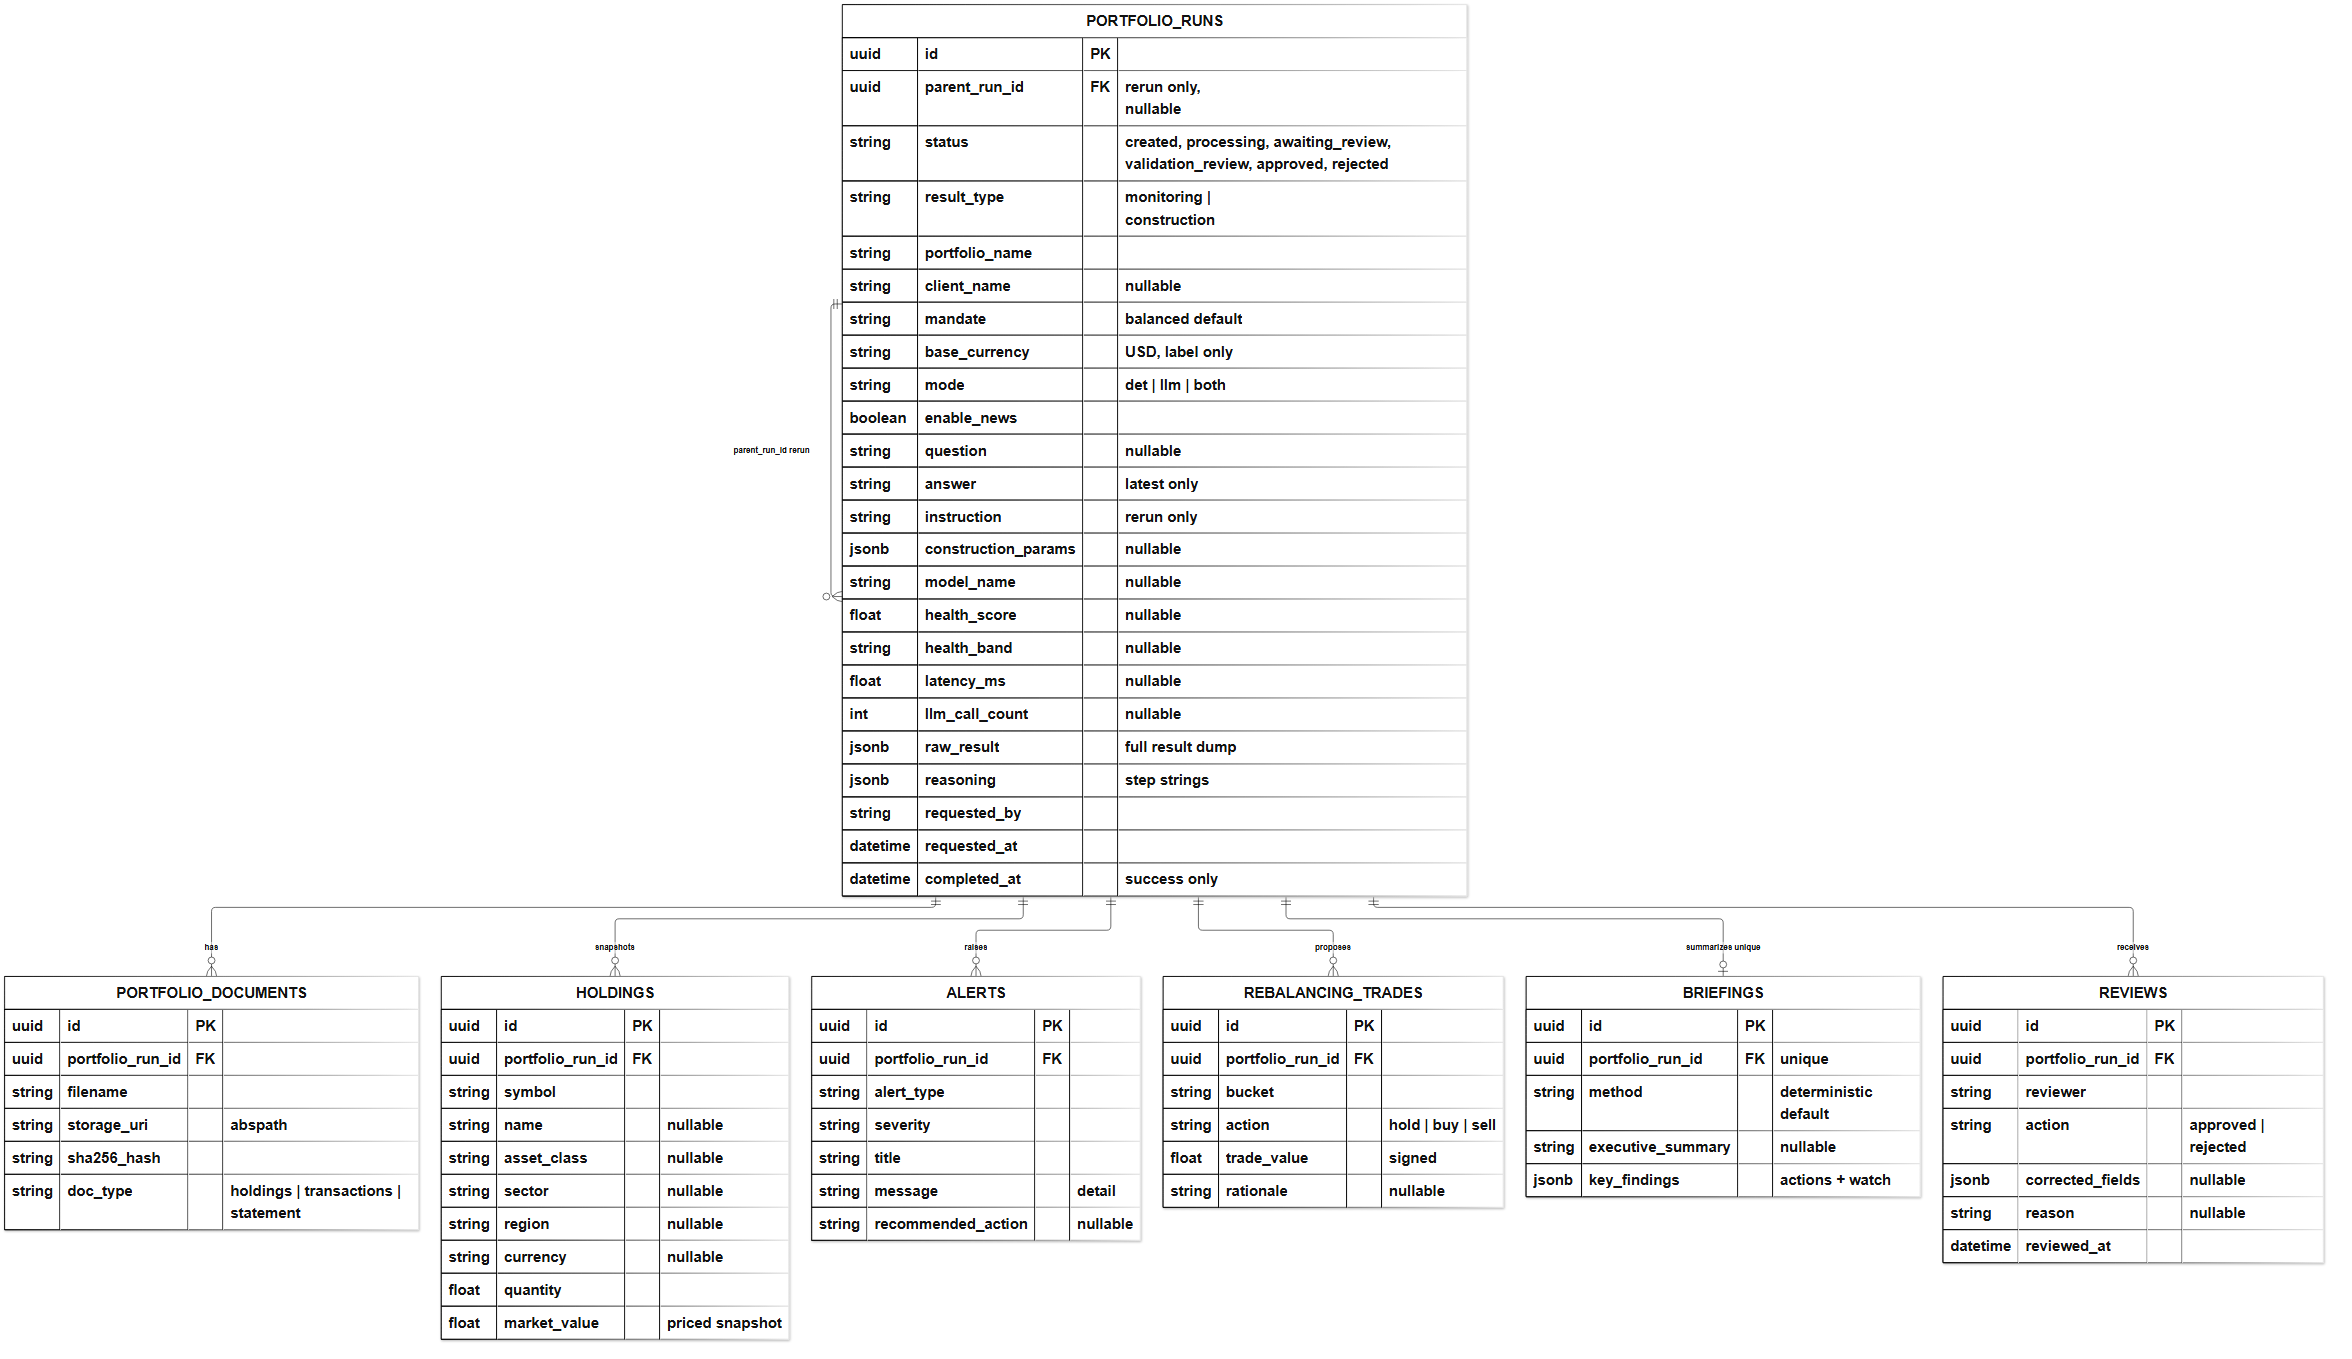
\includegraphics[width=\textwidth,height=0.85\textheight,keepaspectratio]{../diagrams/investment_research/04_erDiagram_10-1-entity-relationship-diagram.png}
\caption{Entity Relationship Diagram}
\label{fig:ch06_investment_research-04-erdiagram-10-1-entity-relationship-diagram}
\end{figure}


\speaker{Interviewer}{The diagram helps. Now detail the run, holdings, alerts, trades, and review tables.}

\subsection{Physical Table Structures}

\subsubsection{Table: \texttt{portfolio\_runs}}

\begin{xltabular}{\textwidth}{>{\raggedright\arraybackslash}X >{\raggedright\arraybackslash}X >{\raggedright\arraybackslash}X >{\raggedright\arraybackslash}X}
\caption{Table: portfolio\_runs}\label{tab:ch06_investment_research-table-portfolio-runs-1}\\
\hline
\textbf{Column} & \textbf{Type} & \textbf{Key / nullable} & \textbf{Description} \\
\hline
\endfirsthead
\caption[]{Table: portfolio\_runs (continued)}\\
\hline
\textbf{Column} & \textbf{Type} & \textbf{Key / nullable} & \textbf{Description} \\
\hline
\endhead
\texttt{id} & UUID & PK & Unique monitoring or construction run \\
\texttt{parent\_run\_id} & UUID & Self-FK, nullable & Links a rerun to its parent \\
\texttt{status} & VARCHAR(32) & Not null & Created, processing, awaiting review, validation review, approved, or rejected \\
\texttt{result\_type} & VARCHAR(20) & Not null & \texttt{monitoring} or \texttt{construction} \\
\texttt{portfolio\_name} & VARCHAR(255) & Not null & Display name \\
\texttt{client\_name} & VARCHAR(255) & Nullable & Optional client label \\
\texttt{mandate} & VARCHAR(64) & Not null & Conservative, balanced, growth, or aggressive \\
\texttt{base\_currency} & VARCHAR(16) & Not null & Currency label; the design does not perform FX conversion \\
\texttt{mode} & VARCHAR(32) & Not null & Deterministic, LLM, or both \\
\texttt{enable\_news} & BOOLEAN & Not null & Whether news and country research are enabled \\
\texttt{question} & TEXT & Nullable & Initial question \\
\texttt{answer} & TEXT & Nullable & Latest Q\&A answer \\
\texttt{instruction} & TEXT & Nullable & Rerun instruction \\
\texttt{construction\_params} & JSONB & Nullable & Original construction request \\
\texttt{model\_name} & VARCHAR(128) & Nullable & LLM model used \\
\texttt{health\_score} & FLOAT & Nullable & Monitoring health score \\
\texttt{health\_band} & VARCHAR(32) & Nullable & Healthy, watch, elevated, or critical \\
\texttt{latency\_ms} & FLOAT & Nullable & End-to-end runtime \\
\texttt{llm\_call\_count} & INTEGER & Nullable & LLM-call count \\
\texttt{raw\_result} & JSONB & Nullable & Full MonitoringResult or ConstructionResult \\
\texttt{reasoning} & JSONB & Nullable & Structured step trace \\
\texttt{requested\_by} & VARCHAR(128) & Not null & Free-text requester identifier \\
\texttt{requested\_at} & TIMESTAMPTZ & Not null & Creation timestamp \\
\texttt{completed\_at} & TIMESTAMPTZ & Nullable & Set on successful completion \\
\hline
\end{xltabular}

\subsubsection{Table: \texttt{portfolio\_documents}}

\begin{xltabular}{\textwidth}{>{\raggedright\arraybackslash}X >{\raggedright\arraybackslash}X >{\raggedright\arraybackslash}X >{\raggedright\arraybackslash}X}
\caption{Table: portfolio\_documents}\label{tab:ch06_investment_research-table-portfolio-documents-2}\\
\hline
\textbf{Column} & \textbf{Type} & \textbf{Key / nullable} & \textbf{Description} \\
\hline
\endfirsthead
\caption[]{Table: portfolio\_documents (continued)}\\
\hline
\textbf{Column} & \textbf{Type} & \textbf{Key / nullable} & \textbf{Description} \\
\hline
\endhead
\texttt{id} & UUID & PK & Document row identifier \\
\texttt{portfolio\_run\_id} & UUID & FK, not null & Owning run \\
\texttt{filename} & VARCHAR(255) & Not null & Original filename \\
\texttt{storage\_uri} & TEXT & Not null & S3 or ADLS object URI of the stored document \\
\texttt{sha256\_hash} & VARCHAR(64) & Not null & Content hash \\
\texttt{doc\_type} & VARCHAR(32) & Not null & Holdings, transactions, or statement \\
\hline
\end{xltabular}

\subsubsection{Table: \texttt{holdings}}

\begin{xltabular}{\textwidth}{>{\raggedright\arraybackslash}X >{\raggedright\arraybackslash}X >{\raggedright\arraybackslash}X >{\raggedright\arraybackslash}X}
\caption{Table: holdings}\label{tab:ch06_investment_research-table-holdings-3}\\
\hline
\textbf{Column} & \textbf{Type} & \textbf{Key / nullable} & \textbf{Description} \\
\hline
\endfirsthead
\caption[]{Table: holdings (continued)}\\
\hline
\textbf{Column} & \textbf{Type} & \textbf{Key / nullable} & \textbf{Description} \\
\hline
\endhead
\texttt{id} & UUID & PK & Holding snapshot ID \\
\texttt{portfolio\_run\_id} & UUID & FK, not null & Owning run \\
\texttt{symbol} & VARCHAR(32) & Not null & Uppercase ticker or identifier \\
\texttt{name} & VARCHAR(255) & Nullable & Company or instrument name \\
\texttt{asset\_class} & VARCHAR(64) & Nullable & Equity, fixed income, cash, alternative, or other \\
\texttt{sector} & VARCHAR(128) & Nullable & Sector label \\
\texttt{region} & VARCHAR(64) & Nullable & Geography or region \\
\texttt{currency} & VARCHAR(16) & Nullable & Instrument currency \\
\texttt{quantity} & FLOAT & Not null & Position quantity \\
\texttt{market\_value} & FLOAT & Nullable & Priced snapshot value \\
\hline
\end{xltabular}

\speaker{Candidate}{That holdings table covers the base columns. Can I note the additional columns, since advisors need price provenance for drift review?}

\speaker{Interviewer}{Yes. What changed?}

\speaker{Candidate}{Persisted holdings store \texttt{price}, \texttt{cost\_basis}, and \texttt{price\_source} with a default of \texttt{input}, so the briefing shows whether a market value came from the uploaded file, live market data, or cost-basis fallback. The full drift lines, risk metrics, cash variances, news scan, country profiles, committee scores, and guardrail corrections live in \texttt{raw\_result} JSONB.}

\subsubsection{Table: \texttt{alerts}}

\begin{xltabular}{\textwidth}{>{\raggedright\arraybackslash}X >{\raggedright\arraybackslash}X >{\raggedright\arraybackslash}X >{\raggedright\arraybackslash}X}
\caption{Table: alerts}\label{tab:ch06_investment_research-table-alerts-4}\\
\hline
\textbf{Column} & \textbf{Type} & \textbf{Key / nullable} & \textbf{Description} \\
\hline
\endfirsthead
\caption[]{Table: alerts (continued)}\\
\hline
\textbf{Column} & \textbf{Type} & \textbf{Key / nullable} & \textbf{Description} \\
\hline
\endhead
\texttt{id} & UUID & PK & Alert identifier \\
\texttt{portfolio\_run\_id} & UUID & FK, not null & Run that raised the alert \\
\texttt{alert\_type} & VARCHAR(64) & Not null & Drift, concentration, limit, cashflow, data quality, or emerging risk \\
\texttt{severity} & VARCHAR(32) & Not null & Low, medium, high, or critical \\
\texttt{title} & VARCHAR(255) & Not null & Short alert title \\
\texttt{message} & TEXT & Not null & Detailed alert content \\
\texttt{recommended\_action} & TEXT & Nullable & Suggested advisor action \\
\hline
\end{xltabular}

\subsubsection{Table: \texttt{rebalancing\_trades}}

\begin{xltabular}{\textwidth}{>{\raggedright\arraybackslash}X >{\raggedright\arraybackslash}X >{\raggedright\arraybackslash}X >{\raggedright\arraybackslash}X}
\caption{Table: rebalancing\_trades}\label{tab:ch06_investment_research-table-rebalancing-trades-5}\\
\hline
\textbf{Column} & \textbf{Type} & \textbf{Key / nullable} & \textbf{Description} \\
\hline
\endfirsthead
\caption[]{Table: rebalancing\_trades (continued)}\\
\hline
\textbf{Column} & \textbf{Type} & \textbf{Key / nullable} & \textbf{Description} \\
\hline
\endhead
\texttt{id} & UUID & PK & Trade-plan row identifier \\
\texttt{portfolio\_run\_id} & UUID & FK, not null & Owning run \\
\texttt{bucket} & VARCHAR(128) & Not null & Sleeve or allocation bucket \\
\texttt{action} & VARCHAR(16) & Not null & Hold, buy, or sell \\
\texttt{trade\_value} & FLOAT & Not null & Signed trade value \\
\texttt{rationale} & TEXT & Nullable & Explanation based on drift and mandate \\
\hline
\end{xltabular}

\subsubsection{Table: \texttt{briefings}}

\begin{xltabular}{\textwidth}{>{\raggedright\arraybackslash}X >{\raggedright\arraybackslash}X >{\raggedright\arraybackslash}X >{\raggedright\arraybackslash}X}
\caption{Table: briefings}\label{tab:ch06_investment_research-table-briefings-6}\\
\hline
\textbf{Column} & \textbf{Type} & \textbf{Key / nullable} & \textbf{Description} \\
\hline
\endfirsthead
\caption[]{Table: briefings (continued)}\\
\hline
\textbf{Column} & \textbf{Type} & \textbf{Key / nullable} & \textbf{Description} \\
\hline
\endhead
\texttt{id} & UUID & PK & Briefing identifier \\
\texttt{portfolio\_run\_id} & UUID & Unique FK & Owning run; one-to-one intended \\
\texttt{method} & VARCHAR(32) & Not null & Deterministic or LLM \\
\texttt{executive\_summary} & TEXT & Nullable & Summary narrative \\
\texttt{key\_findings} & JSONB & Nullable & Stores recommended actions and watch items; name is historical \\
\hline
\end{xltabular}

\speaker{Candidate}{That covers the basic briefing row. Shall I record the split columns so the UI can render sections separately?}

\speaker{Interviewer}{Go ahead.}

\speaker{Candidate}{Briefings store \texttt{allocation\_commentary}, \texttt{risk\_commentary}, and \texttt{cashflow\_commentary} as text plus separate \texttt{recommended\_actions} and \texttt{watch\_items} JSONB arrays. Actions and watch items are stored separately from \texttt{key\_findings}, which is retained only for compatibility. Persist keeps one briefing row per run with a unique run foreign key, and the deterministic narrative is what construction runs store when no LLM briefing exists.}

\subsubsection{Table: \texttt{reviews}}

\begin{xltabular}{\textwidth}{>{\raggedright\arraybackslash}X >{\raggedright\arraybackslash}X >{\raggedright\arraybackslash}X >{\raggedright\arraybackslash}X}
\caption{Table: reviews}\label{tab:ch06_investment_research-table-reviews-7}\\
\hline
\textbf{Column} & \textbf{Type} & \textbf{Key / nullable} & \textbf{Description} \\
\hline
\endfirsthead
\caption[]{Table: reviews (continued)}\\
\hline
\textbf{Column} & \textbf{Type} & \textbf{Key / nullable} & \textbf{Description} \\
\hline
\endhead
\texttt{id} & UUID & PK & Review identifier \\
\texttt{portfolio\_run\_id} & UUID & FK, not null & Reviewed run \\
\texttt{reviewer} & VARCHAR(128) & Not null & Reviewer identity; no authentication in the design \\
\texttt{action} & VARCHAR(16) & Not null & Approved, rejected, or corrected \\
\texttt{corrected\_fields} & JSONB & Nullable & Corrections supplied by reviewer \\
\texttt{reason} & TEXT & Nullable & Review explanation \\
\texttt{reviewed\_at} & TIMESTAMPTZ & Not null & Review timestamp \\
\hline
\end{xltabular}


\speaker{Candidate}{Tables are defined. Shall I note the join paths from runs to holdings, alerts, and briefings?}

\subsection{Join Paths Readers Should Remember}

\begin{xltabular}{\textwidth}{>{\raggedright\arraybackslash}X >{\raggedright\arraybackslash}X >{\raggedright\arraybackslash}X >{\raggedright\arraybackslash}X}
\caption{Join Paths Readers Should Remember}\label{tab:ch06_investment_research-10-3-join-paths-readers-should-remember-8}\\
\hline
\textbf{From} & \textbf{To} & \textbf{Join condition} & \textbf{Why it matters} \\
\hline
\endfirsthead
\caption[]{Join Paths Readers Should Remember (continued)}\\
\hline
\textbf{From} & \textbf{To} & \textbf{Join condition} & \textbf{Why it matters} \\
\hline
\endhead
\texttt{portfolio\_runs} & \texttt{portfolio\_documents} & \texttt{portfolio\_runs.id = portfolio\_documents.portfolio\_run\_id} & Identify uploaded inputs \\
\texttt{portfolio\_runs} & \texttt{holdings} & \texttt{portfolio\_runs.id = holdings.portfolio\_run\_id} & Load position snapshot \\
\texttt{portfolio\_runs} & \texttt{alerts} & \texttt{portfolio\_runs.id = alerts.portfolio\_run\_id} & Load risk and action alerts \\
\texttt{portfolio\_runs} & \texttt{rebalancing\_trades} & \texttt{portfolio\_runs.id = rebalancing\_trades.portfolio\_run\_id} & Load proposed trades \\
\texttt{portfolio\_runs} & \texttt{briefings} & \texttt{portfolio\_runs.id = briefings.portfolio\_run\_id} & Load deterministic or LLM briefing \\
\texttt{portfolio\_runs} & \texttt{reviews} & \texttt{portfolio\_runs.id = reviews.portfolio\_run\_id} & Load review history \\
\texttt{portfolio\_runs} & \texttt{portfolio\_runs} & \texttt{child.parent\_run\_id = parent.id} & Traverse rerun lineage \\
\hline
\end{xltabular}


\speaker{Interviewer}{How do those tables flow into the advisor UI views?}

\subsection{Data Flow from Tables to UI}

\begin{figure}[htbp]
\centering
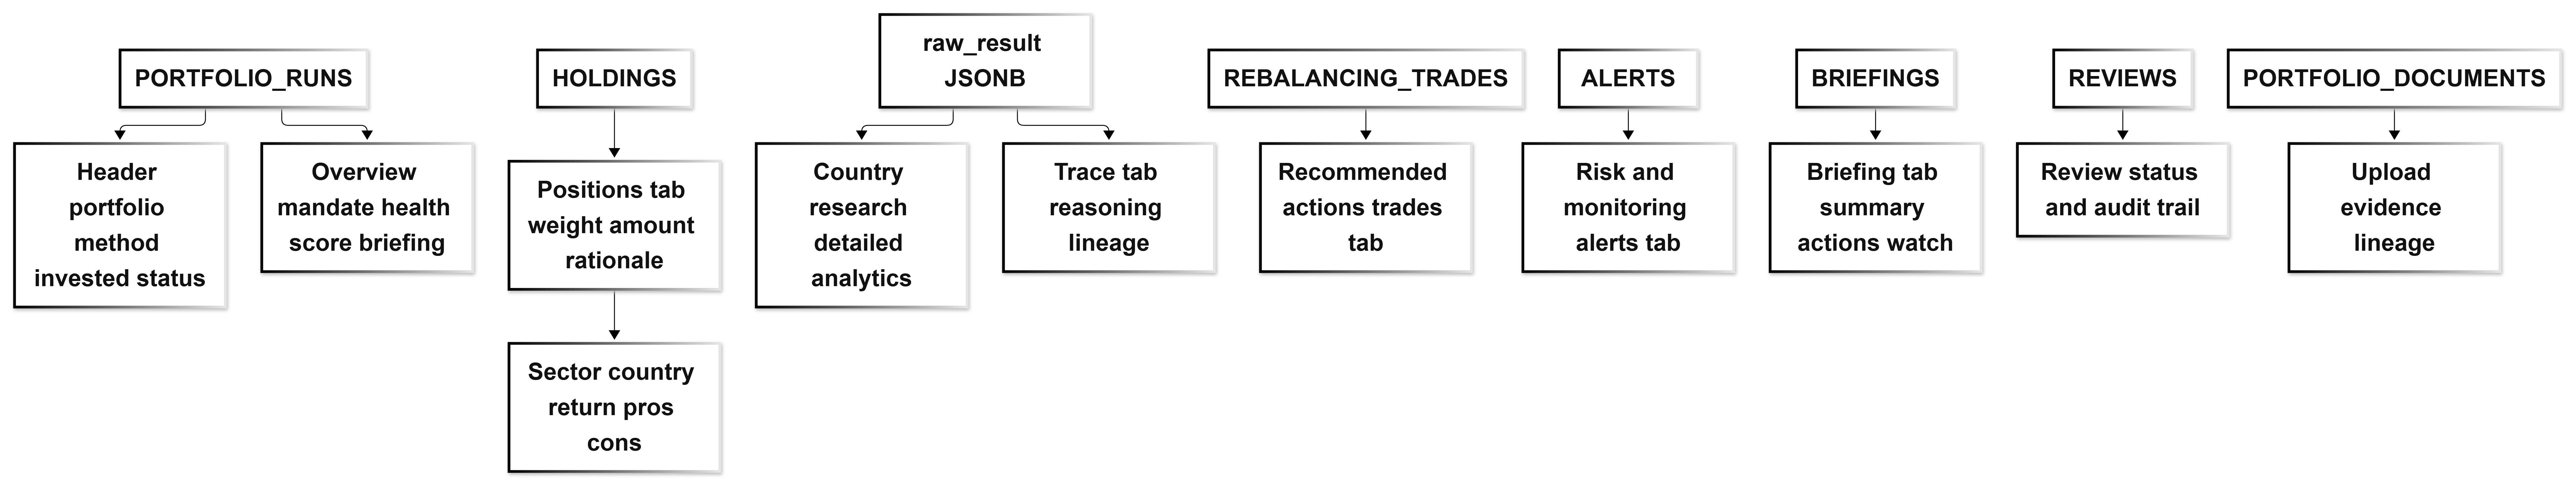
\includegraphics[width=\textwidth,height=0.85\textheight,keepaspectratio]{../diagrams/investment_research/05_flowchart_10-4-data-flow-from-tables-to-ui.png}
\caption{Data Flow from Tables to UI}
\label{fig:ch06_investment_research-05-flowchart-10-4-data-flow-from-tables-to-ui}
\end{figure}


\speaker{Candidate}{The UI mapping is clear. Shall I state the modeling principles --- reruns as children, raw result retained?}

\subsection{Modeling Principles}

\speaker{Candidate}{I would follow these principles:}

\begin{enumerate}[leftmargin=\speakwid]
\item One \texttt{portfolio\_runs} row represents one reproducible analysis run.
\item Reruns create a new child run instead of mutating the parent.
\item Holdings, alerts, trades, briefings, and reviews are directly scoped to the run.
\item Core operational objects are normalized for queries, while the complete result remains in \texttt{raw\_result}.
\item Construction and monitoring reuse the same run anchor and child tables.
\item Numeric decisions are stored after deterministic recomputation, not directly from LLM output.
\item Review records represent human workflow state, not automatic trade execution.
\end{enumerate}
\speaker{Interviewer}{Why retain the whole result in JSON if the child tables already exist?}

\speaker{Candidate}{The child tables support common operational queries. The JSON preserves richer objects such as drift lines, risk metrics, country research profiles, committee scores, feasibility, comparison, and guardrail corrections without requiring a schema migration for every new analytical field.}


\speaker{Interviewer}{Show me how the advisor sees holdings, country research, and trace in the product screens.}

\medskip\hrule\medskip
\section{Product Screens and Reader Walkthrough}
\label{sec:ch06_investment_research-11-product-screens-and-reader-walkthrough}

The product UI exposes the workflow through a left-side control panel and a result area with four tabs: Overview, Positions, Country research, and Trace.

\subsection{Overview View}

The header shows portfolio name, construction or monitoring method, invested amount, and status. The Overview tab contains the mandate, category, weighting method, sleeve targets, expected-return projection, and summary narrative.

It also includes a follow-up question box and a rerun section where the advisor can retain or override mandate, target, and related parameters.


\begin{figure}[htbp]
\centering
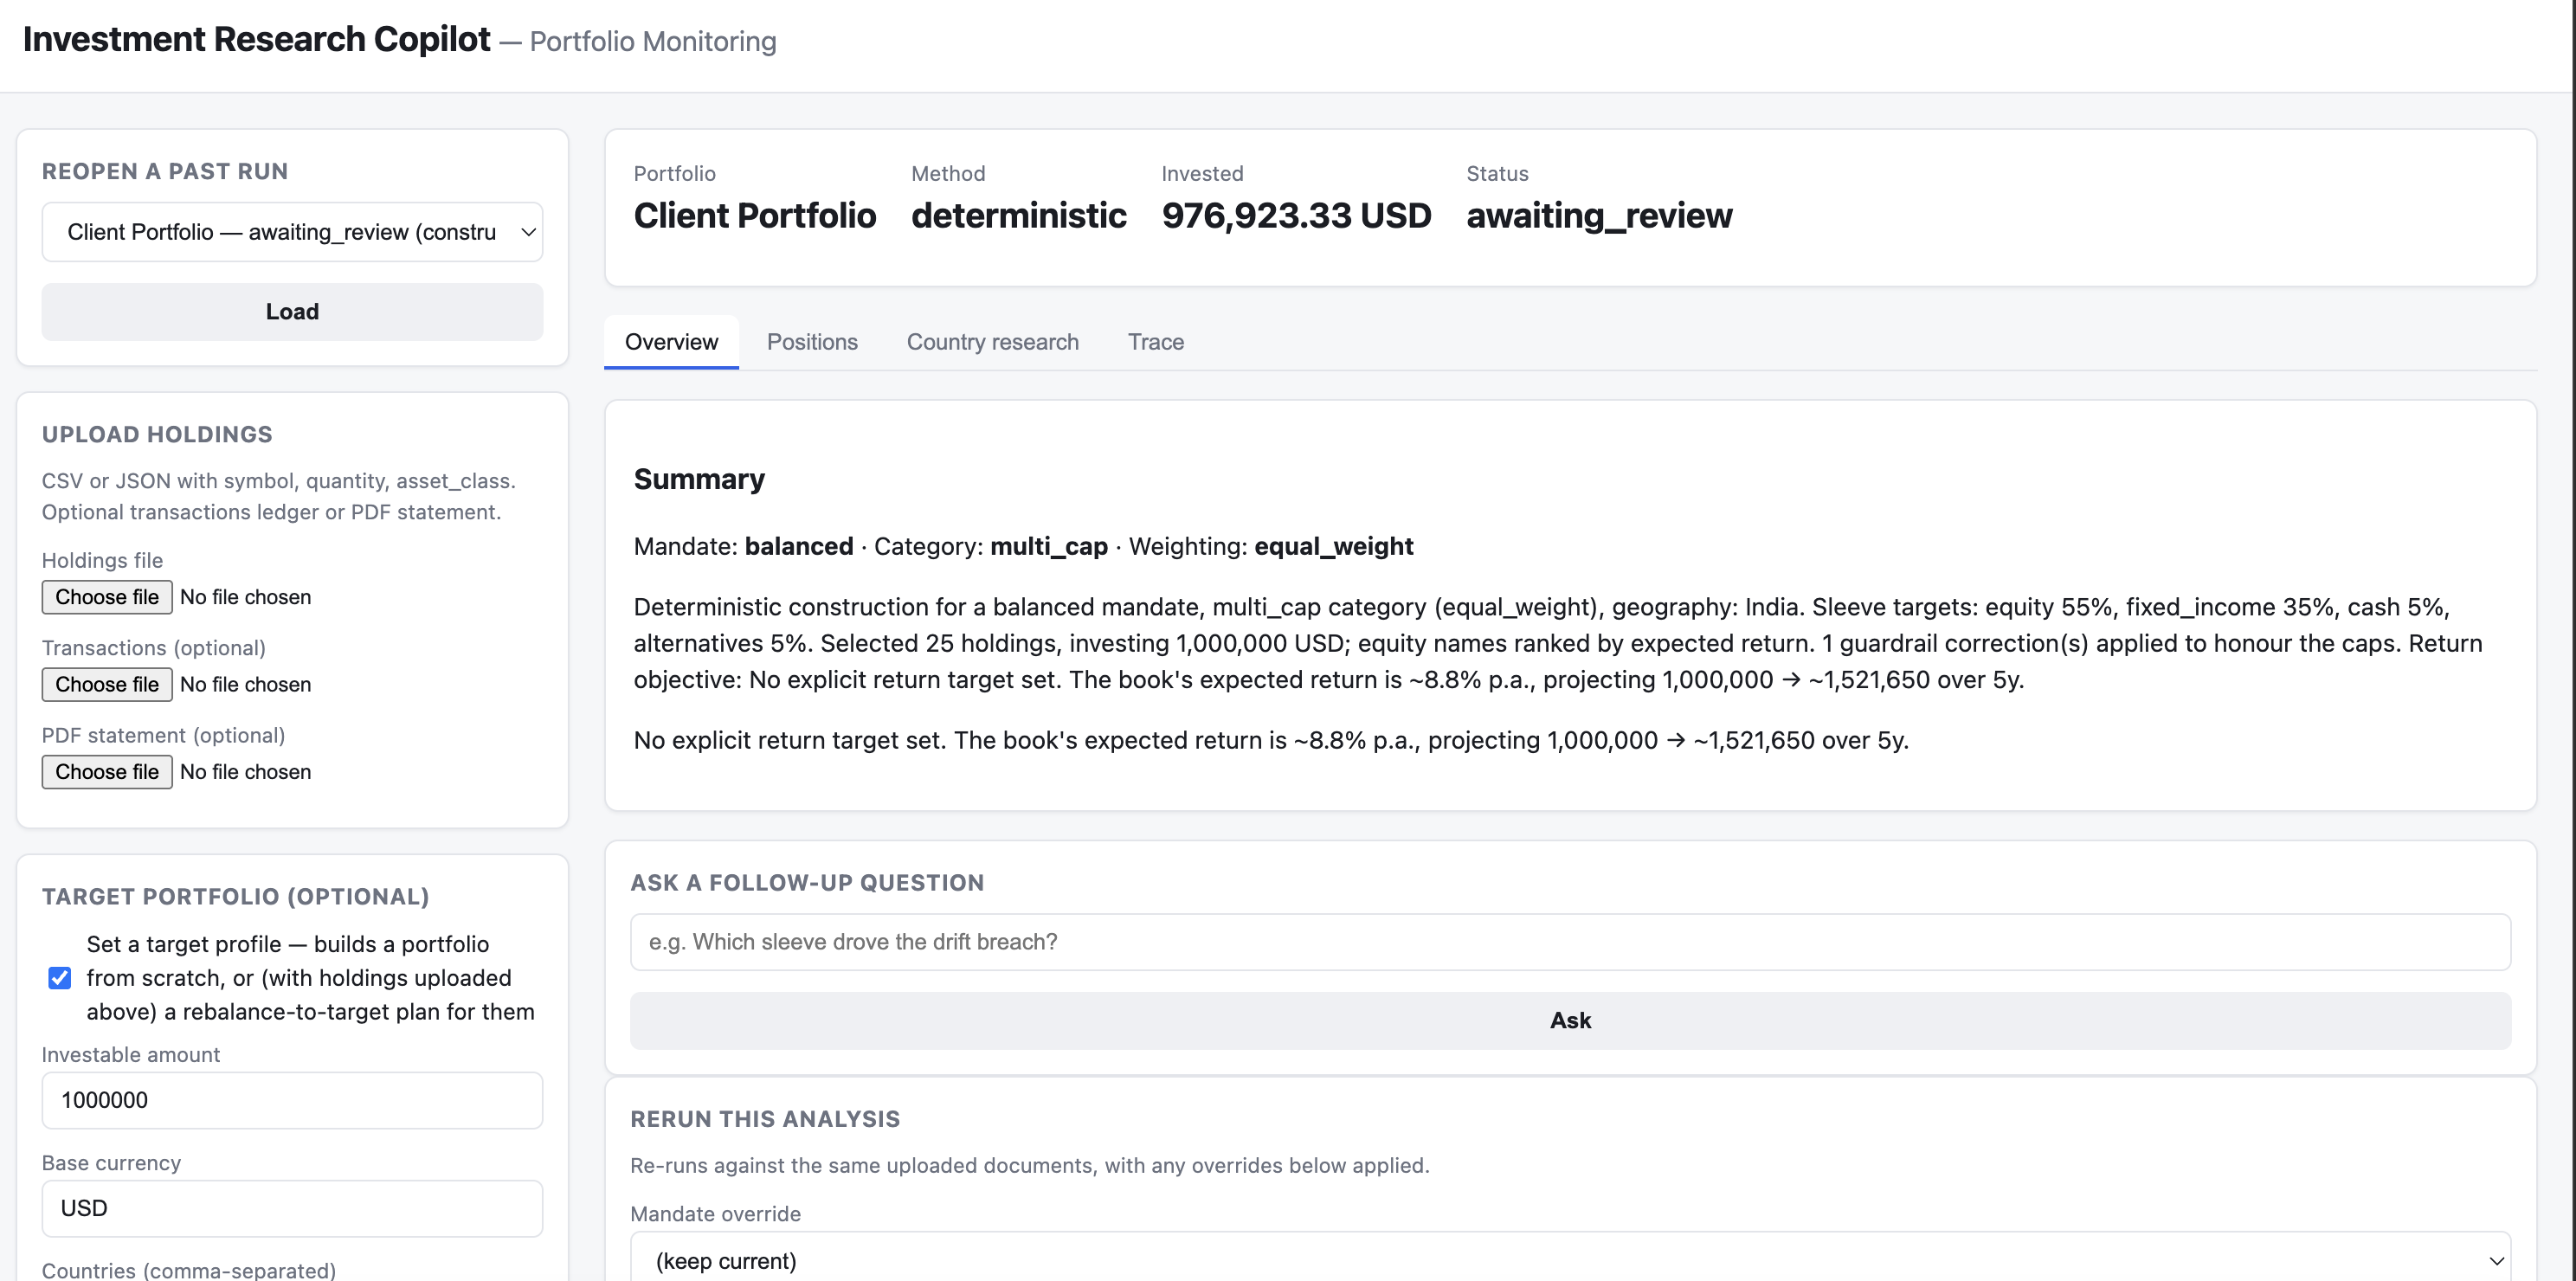
\includegraphics[width=\textwidth,height=0.85\textheight,keepaspectratio]{../diagrams/investment_research/screen_11_1_overview.png}
\caption{Overview view: portfolio header, mandate summary, expected-return projection, and follow-up controls.}
\label{fig:ch06_investment_research-screen-11-1-overview}
\end{figure}


\speaker{Candidate}{Overview is clear. Shall we inspect positions --- weights, amounts, and selection reasons?}

\subsection{Positions View}

The Positions tab displays:

\begin{itemize}[leftmargin=\speakwid]
\item Symbol.
\item Category or sector.
\item Country.
\item Portfolio weight.
\item Invested amount.
\item Expected return.
\item Selection reason.
\end{itemize}
For a deterministic construction, rows may show sleeve reasoning such as equal weight across selected names, sector diversification, large-cap selection, and expected-return ranking.


\begin{figure}[htbp]
\centering
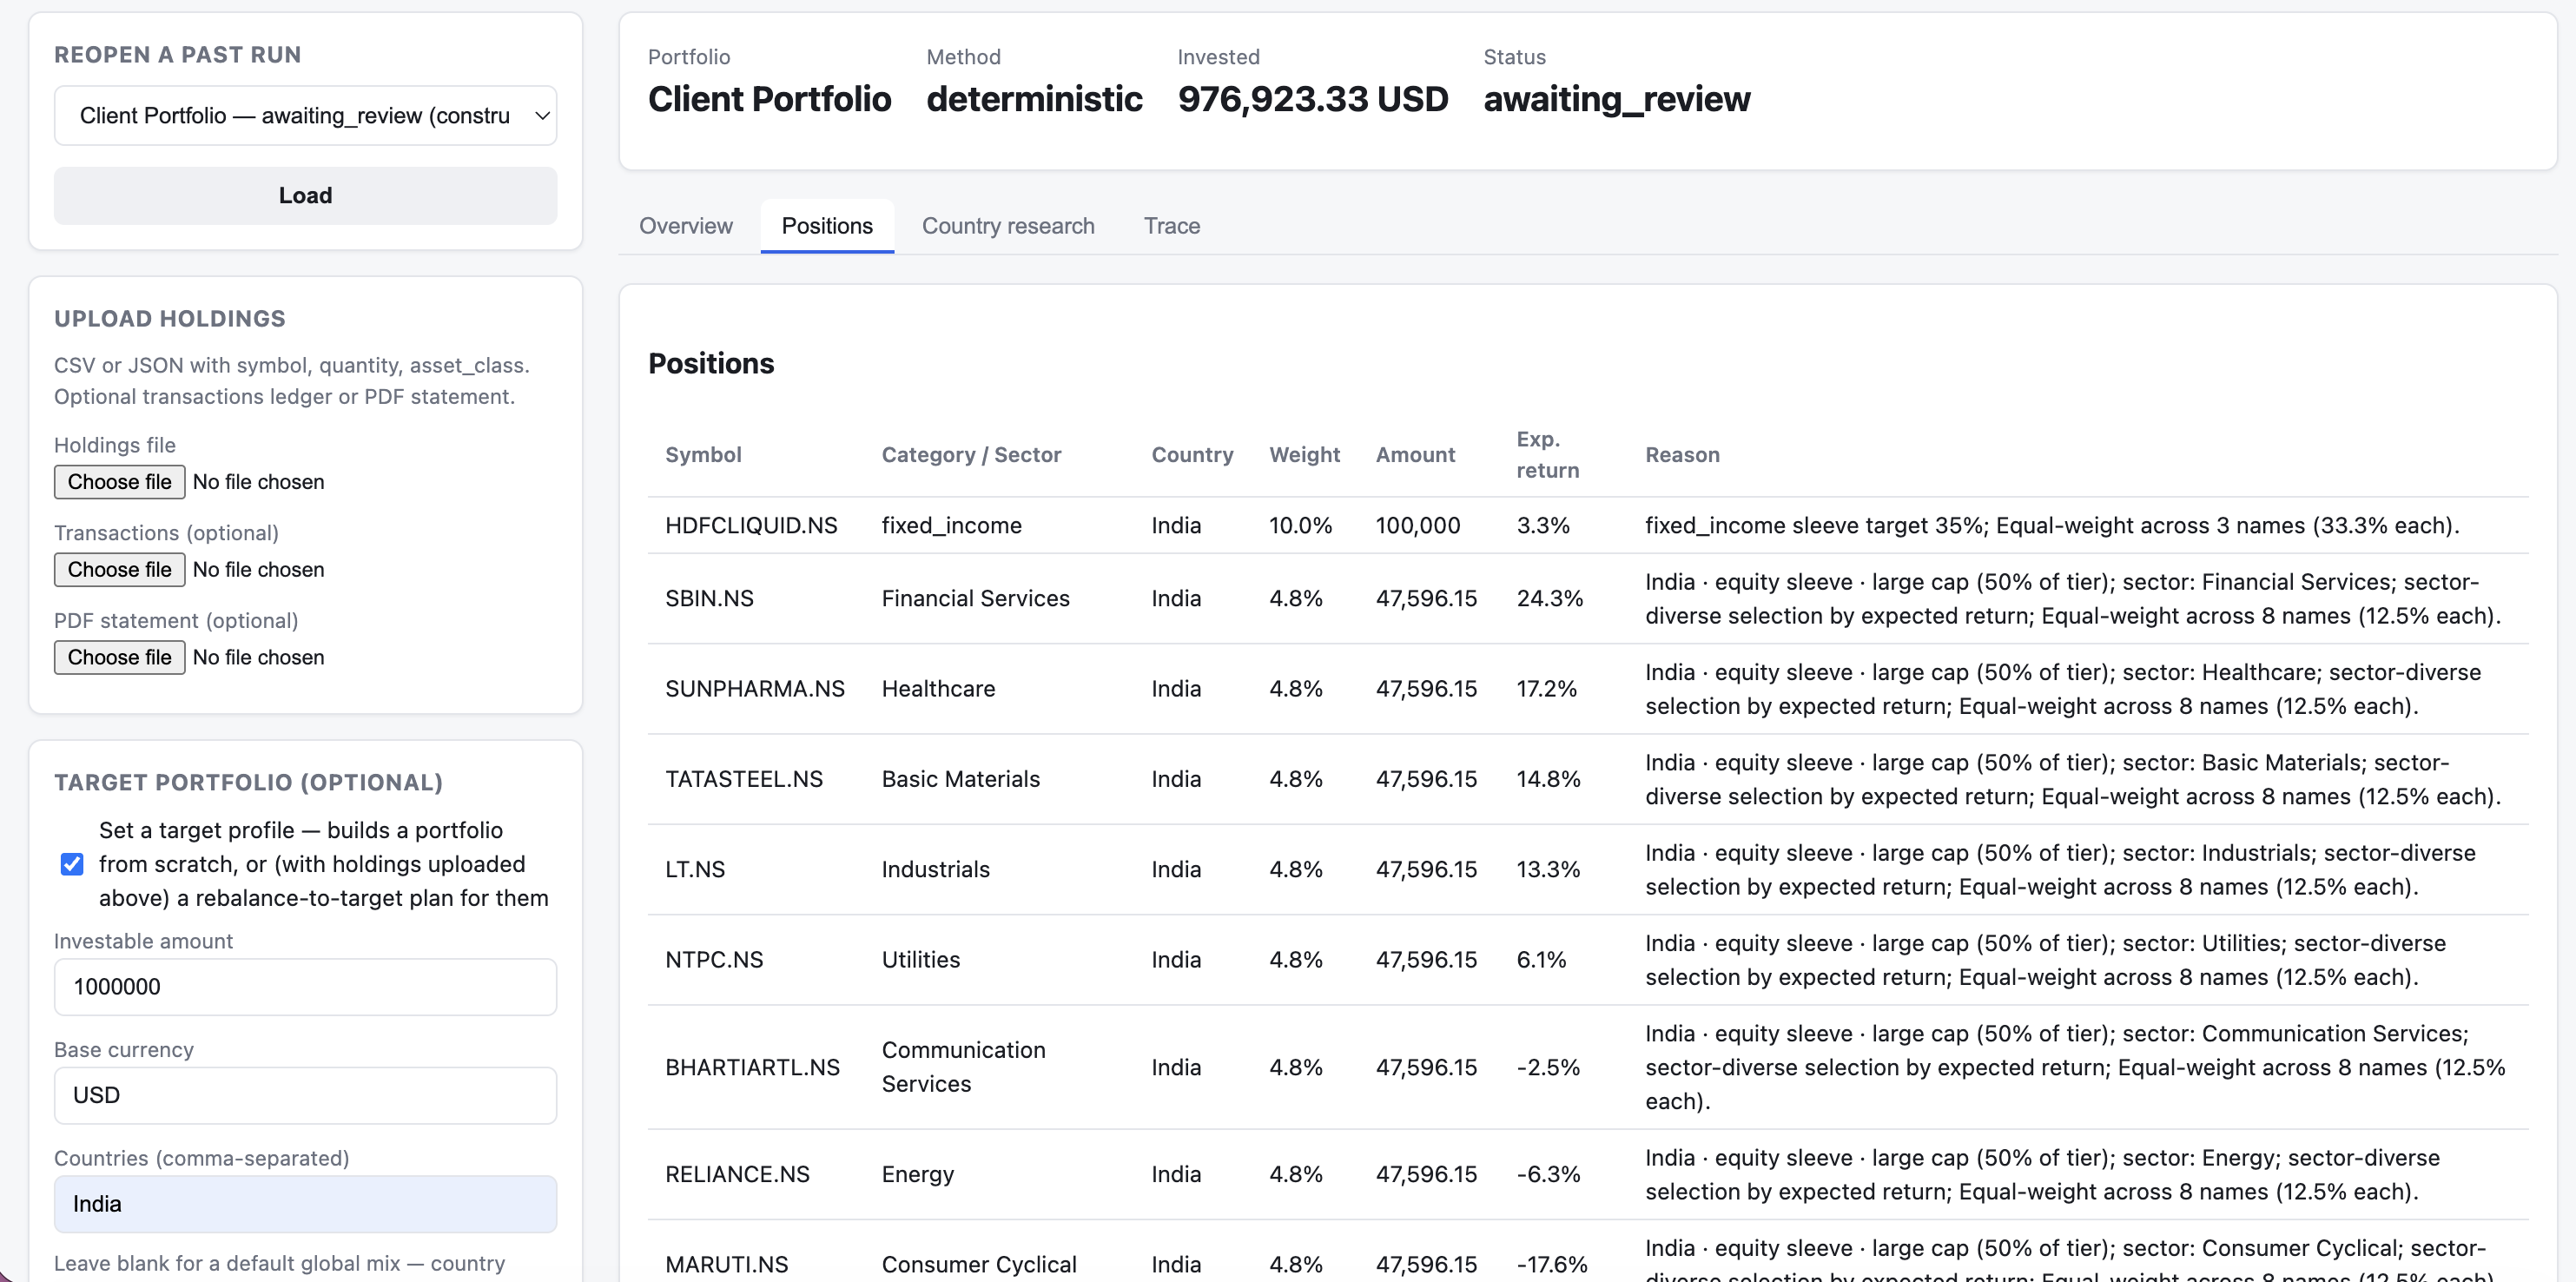
\includegraphics[width=\textwidth,height=0.85\textheight,keepaspectratio]{../diagrams/investment_research/screen_11_2_positions.png}
\caption{Positions view: holdings with weight, invested amount, expected return, and selection reason.}
\label{fig:ch06_investment_research-screen-11-2-positions}
\end{figure}


\speaker{Interviewer}{How does the country research view present severity without overriding limits?}

\subsection{Country Research View}

The Country research tab displays the country profile, an overall severity label, deposit or fixed-income rate context, bond-credit proxy, and research findings categorized by fixed income, geopolitical, market, and sector risks.

Country research is contextual. It should inform monitoring and committee commentary but should not override deterministic allocation limits or trade rules.


\begin{figure}[htbp]
\centering
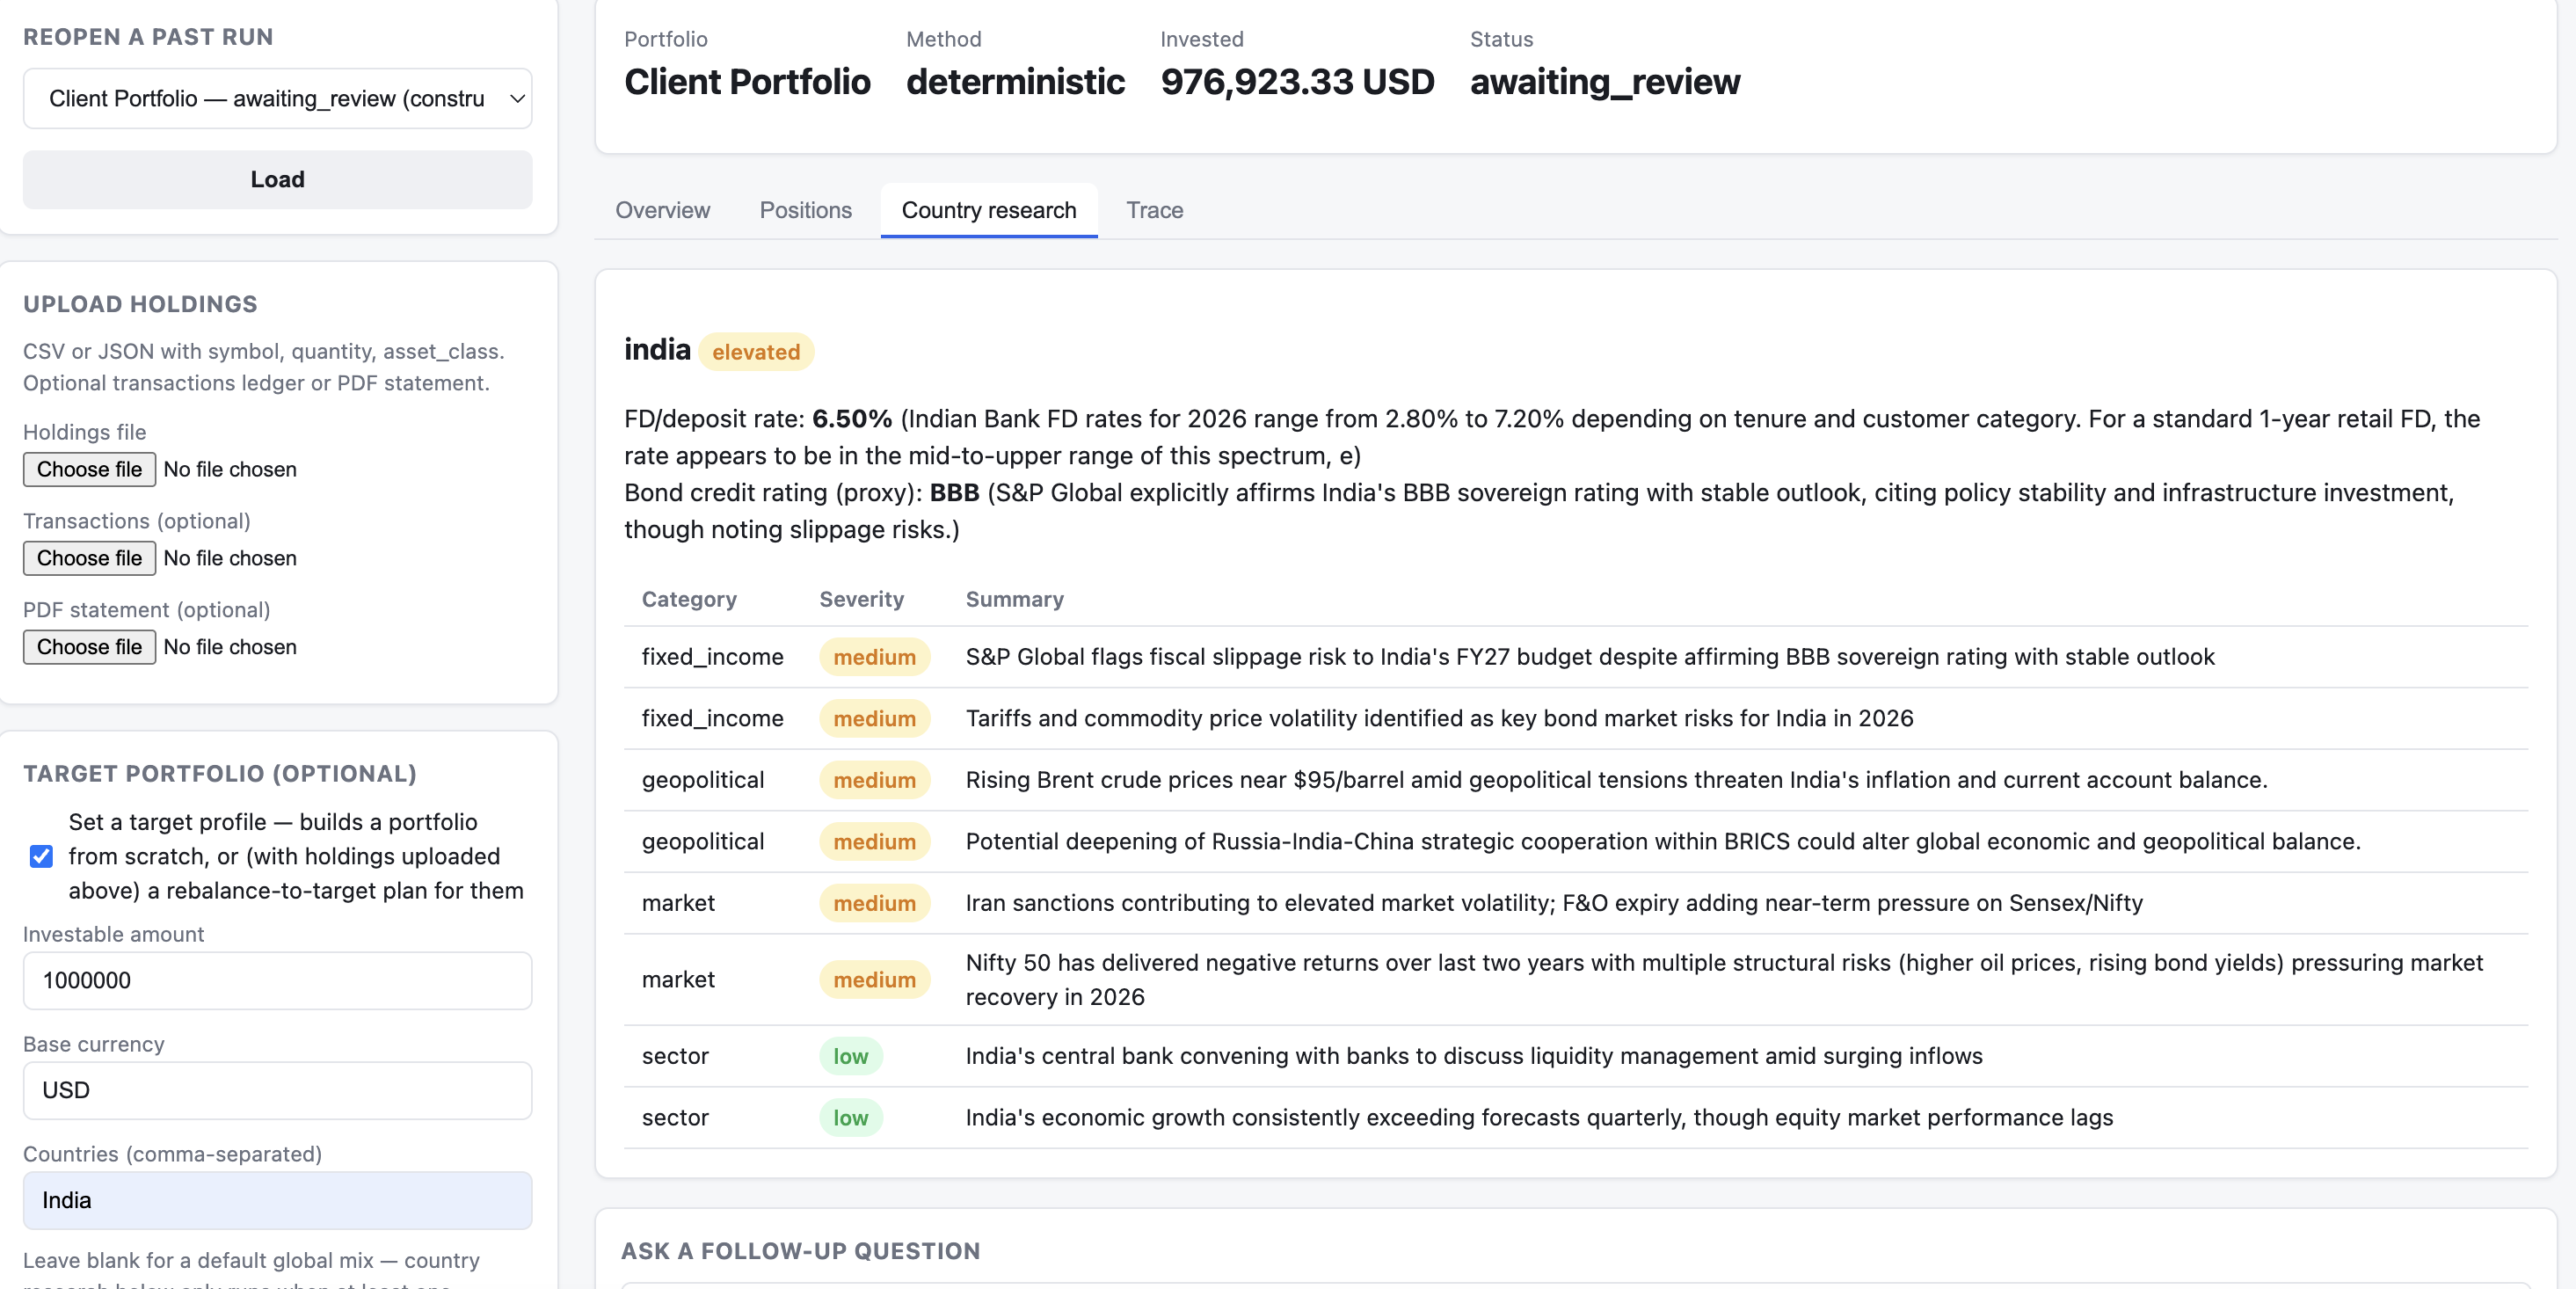
\includegraphics[width=\textwidth,height=0.85\textheight,keepaspectratio]{../diagrams/investment_research/screen_11_3_country_research.png}
\caption{Country research view: country profile, severity label, and categorized research findings.}
\label{fig:ch06_investment_research-screen-11-3-country-research}
\end{figure}


\speaker{Candidate}{Country context stays capped. Shall we open the trace behind each trade and alert?}

\subsection{Trace View}

The Trace tab is intended to expose computation steps, research evidence, data sources, model metadata, and decision reasoning. This is especially useful when an advisor asks why a trade, alert, or position appears in the result.


\speaker{Interviewer}{What controls let the advisor reopen runs and switch monitoring versus construction?}

\subsection{User-Control Panel}

The left panel supports:

\begin{itemize}[leftmargin=\speakwid]
\item Reopening a past run.
\item Uploading holdings.
\item Uploading transactions.
\item Uploading a PDF statement.
\item Setting a target portfolio.
\item Choosing investable amount and base currency.
\item Entering countries and construction constraints.
\end{itemize}
The controls make the distinction between monitoring an existing portfolio and constructing a target portfolio visible to the user.


\speaker{Interviewer}{How would you evaluate holdings ingestion, drift, risk, guardrails, and briefings end to end?}

\medskip\hrule\medskip
\section{Evaluation Framework}
\label{sec:ch06_investment_research-12-evaluation-framework}

\speaker{Interviewer}{How would you evaluate the complete system?}

\speaker{Candidate}{I would evaluate it in layers.}

\subsection{Ingestion Evaluation}

\begin{itemize}[leftmargin=\speakwid]
\item CSV and JSON alias-mapping correctness.
\item Invalid-row handling.
\item PDF statement transcription precision.
\item Quantity, price, and market-value fidelity.
\item Transaction-type normalization.
\end{itemize}

\speaker{Candidate}{Ingestion checks pass. Shall we verify pricing, allocation, and coverage next?}

\subsection{Market and Allocation Evaluation}

\begin{itemize}[leftmargin=\speakwid]
\item Price-source priority correctness.
\item Market-value correctness.
\item Allocation weights against a reference implementation.
\item Data-coverage accuracy.
\item Asset-class, sector, country, and currency aggregation correctness.
\end{itemize}

\speaker{Interviewer}{How do you verify drift bands, trade values, and ledger reconciliation?}

\subsection{Drift and Cash-Flow Evaluation}

\begin{itemize}[leftmargin=\speakwid]
\item Target and band mapping.
\item Breach classification.
\item Trade-value correctness.
\item Turnover and estimated transaction-cost correctness.
\item Expected-income calculations.
\item Actual-ledger reconciliation.
\item Missing, shortfall, excess, and unexpected-flow classification.
\end{itemize}

\speaker{Candidate}{Cash flows reconcile. How do we validate risk metrics, limits, and health reproducibility?}

\subsection{Risk and Alert Evaluation}

\begin{itemize}[leftmargin=\speakwid]
\item Volatility, drawdown, VaR, beta, tracking error, HHI, and effective-N correctness.
\item Limit-check correctness.
\item Alert severity ordering.
\item News and country risk discount behavior.
\item Health-score reproducibility.
\end{itemize}

\speaker{Interviewer}{How do you evaluate universe filtering, committee scores, and cap enforcement?}

\subsection{Construction Evaluation}

\begin{itemize}[leftmargin=\speakwid]
\item Universe filtering correctness.
\item Committee-score reproducibility.
\item Deterministic selection and weighting correctness.
\item LLM candidate whitelist enforcement.
\item Single-name and sector-cap enforcement.
\item Repricing and share-count correctness.
\item Feasibility classification.
\item Deterministic-versus-LLM comparison correctness.
\end{itemize}

\speaker{Candidate}{Construction math holds. How do we check briefings and Q\&A stay grounded?}

\subsection{Narrative Evaluation}

\begin{itemize}[leftmargin=\speakwid]
\item Briefing completeness.
\item Consistency with computed metrics.
\item Unsupported-number rate.
\item Quality of recommended actions.
\item Q\&A factual correctness.
\item Position annotation grounding.
\end{itemize}

\speaker{Interviewer}{Finally, how do you test reruns, reviews, audit traces, and graceful failures?}

\subsection{Workflow Evaluation}

\begin{itemize}[leftmargin=\speakwid]
\item Successful completion rate.
\item Processing latency.
\item Celery and BackgroundTasks parity.
\item Rerun lineage correctness.
\item Review-state correctness.
\item Audit-trace completeness.
\item Recovery from Redis, market-data, news, and LLM failures.
\end{itemize}
\speaker{Interviewer}{How would you create a golden dataset?}

\speaker{Candidate}{I would prepare portfolios with known prices, histories, target mandates, transaction ledgers, news fixtures, and expected outputs. The dataset should include concentration breaches, drift breaches, missing prices, short history, large cash flows, multiple currencies, infeasible construction constraints, LLM-generated invalid tickers, and failed external services.}


\speaker{Candidate}{Evaluation is covered. Shall we stress-test the failure modes --- missing prices, drift breaches, and reruns?}

\medskip\hrule\medskip
\section{Edge Cases and Failure Scenarios}
\label{sec:ch06_investment_research-13-edge-cases-and-failure-scenarios}

\speaker{Interviewer}{Let us stress test the design.}

\subsection{Case 1: No Holdings File and No Statement}

\speaker{Interviewer}{What happens if the user submits neither holdings nor a statement PDF?}

\speaker{Candidate}{The route can raise a \texttt{ValueError}, which may become an HTTP 500. That should be fixed to return a clear 400 validation response stating that one holdings source is required.}


\speaker{Candidate}{Missing inputs fail clearly. What about an invalid holdings row?}

\subsection{Case 2: Invalid Holdings Row}

\speaker{Interviewer}{A row has quantity but no symbol. What happens?}

\speaker{Candidate}{The row should be rejected or reported as invalid. The system must not create a position with an empty symbol.}


\speaker{Interviewer}{A holding has no price anywhere. What then?}

\subsection{Case 3: Missing Price}

\speaker{Interviewer}{A holding has no input price and yfinance cannot find a quote.}

\speaker{Candidate}{The system can use cost basis divided by quantity if available. Otherwise it marks the holding unpriced, excludes it from priced allocation totals, lowers coverage, and raises a data-quality alert.}


\speaker{Candidate}{Unpriced holdings are flagged. What if history is too short for risk?}

\subsection{Case 4: Missing Market History}

\speaker{Interviewer}{A new instrument has only five days of history.}

\speaker{Candidate}{Metrics requiring longer history become unavailable. The system should not infer volatility or VaR from insufficient data. The result should show the coverage limitation.}


\speaker{Interviewer}{Equity breaches its mandate band. What trade results?}

\subsection{Case 5: Portfolio Breaches Equity Target}

\speaker{Interviewer}{Equity is at 68 percent while the balanced target is 55 percent with a 5-point band. What happens?}

\speaker{Candidate}{The sleeve is above the 60 percent upper band. The drift engine creates a breach-over line and a sell trade sized toward the target. The alert recommends reviewing or executing the rebalance, but no trade is placed automatically.}


\speaker{Candidate}{Breach sizing is clear. How is income reported with no ledger?}

\subsection{Case 6: No Transaction Ledger}

\speaker{Interviewer}{How do you report income when no ledger is uploaded?}

\speaker{Candidate}{The system reports expected income only and explicitly labels actual income as unavailable. It should not create a false shortfall from missing observations.}


\speaker{Interviewer}{A large unrelated withdrawal lands in the ledger. How is it classified?}

\subsection{Case 7: Unexpected Withdrawal}

\speaker{Interviewer}{A large withdrawal appears in the ledger but is unrelated to held securities.}

\speaker{Candidate}{It is classified as an unexpected flow. If it exceeds the configured absolute threshold, it receives higher severity and becomes an alert for advisor review.}


\speaker{Candidate}{Cash flows are classified. What if the news provider is down?}

\subsection{Case 8: News Provider Failure}

\speaker{Interviewer}{DuckDuckGo is unavailable during monitoring.}

\speaker{Candidate}{The run continues. The news scan returns a data gap or keyword fallback result, and deterministic limits and scores remain unaffected.}


\speaker{Interviewer}{A country research node fails mid-run. Does monitoring block?}

\subsection{Case 9: Country Research Failure}

\speaker{Interviewer}{One country research node fails.}

\speaker{Candidate}{Country research is fail-soft. The profile can be partial or empty, and the run should continue with a research-gap note. It must not block allocation or risk calculations.}


\speaker{Candidate}{Research gaps are marked. What if the LLM invents a ticker?}

\subsection{Case 10: LLM Invents a Ticker}

\speaker{Interviewer}{The LLM constructor returns a symbol outside the universe.}

\speaker{Candidate}{The whitelist removes it. If too few positions remain, the result should show the correction or fallback and may retain residual cash rather than inventing another security.}


\speaker{Interviewer}{The user sets incompatible caps and minimums. How do guardrails respond?}

\subsection{Case 11: Guardrail-Infeasible Portfolio}

\speaker{Interviewer}{The user requests ten percent minimum positions but also allows only five percent single-name caps. What happens?}

\speaker{Candidate}{The guardrail algorithm detects infeasibility, caps positions, redistributes where possible, and records corrections or residual cash. It should not claim that all requested constraints were satisfied if they are mathematically incompatible.}


\speaker{Candidate}{Infeasibility is disclosed. How are cross-currency holdings handled without FX conversion?}

\subsection{Case 12: Cross-Currency Portfolio}

\speaker{Interviewer}{The portfolio contains USD, INR, and EUR assets but base currency is USD.}

\speaker{Candidate}{The design labels the base currency but does not convert FX. The result should disclose that limitation. A production system needs FX rates, conversion timestamps, and currency-risk treatment.}


\speaker{Interviewer}{News flags a name but limits are fine. Does the band flip?}

\subsection{Case 13: News Says a Company Has a Problem but Limit Checks Are Fine}

\speaker{Interviewer}{Should emerging news automatically make the portfolio critical?}

\speaker{Candidate}{No. News and country findings are discounted and capped at medium. They create context and watch alerts but should not override deterministic risk limits or dominate the health score.}


\speaker{Candidate}{News stays capped. What if a stored object is missing at rerun?}

\subsection{Case 14: Re-run After Uploaded Files Are Deleted}

\speaker{Interviewer}{What if an uploaded object has been deleted from S3 or ADLS before a rerun?}

\speaker{Candidate}{The rerun must fail clearly when a source object is missing. Document URIs point to versioned objects in durable storage, so the API validates source availability before scheduling a rerun.}


\speaker{Interviewer}{A reviewer corrects a classification. Does the score recompute?}

\subsection{Case 15: Review Correction}

\speaker{Interviewer}{A reviewer corrects a sector classification. Does the score automatically update?}

\speaker{Candidate}{No. The review endpoint records corrected fields but does not recompute the result. A corrected child run should explicitly trigger recomputation so the displayed result and correction do not diverge.}


\speaker{Candidate}{Corrections are recorded. What stops a bogus portfolio ID from polling cleanly?}

\subsection{Case 16: Bogus Portfolio ID}

\speaker{Interviewer}{What if a user polls a random portfolio ID?}

\speaker{Candidate}{Redis-first status behavior may return a processing-like response for an unknown ID. The endpoint should verify the run exists in Postgres before returning a valid lifecycle state.}


\speaker{Candidate}{Failure handling is clear. Shall we discuss deployment --- API replicas, Postgres, Redis, and S3 storage?}

\medskip\hrule\medskip
\section{Deployment and Operations}
\label{sec:ch06_investment_research-14-deployment-and-operations}

\speaker{Interviewer}{How would you deploy this system?}

\speaker{Candidate}{I would begin with one API replica, Postgres, Redis, and S3 or ADLS object storage. Locally, BackgroundTasks is sufficient. In a larger environment, I would run Celery workers with Redis DB 1 as broker/backend and use Redis DB 0 for live phases.}

\subsection{Current Operational Shape}

\begin{itemize}[leftmargin=\speakwid]
\item One FastAPI service.
\item Vanilla JavaScript production UI.
\item Optional Streamlit development UI.
\item Postgres database.
\item Redis for phases and optional Celery.
\item S3 or ADLS object storage for uploads.
\item BackgroundTasks or Celery.
\item External market and research providers.
\item Optional LLM gateway.
\end{itemize}

\speaker{Interviewer}{Why start with a single replica when files already sit in durable storage?}

\subsection{Why Single Replica Matters}

\speaker{Candidate}{Uploaded documents live in S3 or ADLS and reruns reuse those durable URIs, so any replica or worker can locate the same files. The deployment stays a single service at first for simplicity.}

\speaker{Interviewer}{What must change for horizontal scaling?}

\speaker{Candidate}{Add a durable queue, make jobs idempotent, and scale API and worker replicas independently against shared object storage and Postgres.}


\speaker{Candidate}{Scaling is planned. Which API, job, market-data, and review signals need monitoring?}

\subsection{Monitoring Needs}

\begin{itemize}[leftmargin=\speakwid]
\item API request and response metrics.
\item Background and Celery job durations.
\item Redis phase availability.
\item Market-data success and coverage.
\item News-provider success and latency.
\item LLM calls, tokens, and errors.
\item Portfolio calculation failures.
\item Alert and health-band distribution.
\item Guardrail correction counts.
\item Review and rerun frequency.
\item Storage and database failures.
\end{itemize}

\speaker{Interviewer}{What gaps remain in holdings coverage, risk, guardrails, and review before production?}

\medskip\hrule\medskip
\section{Current Gaps and Enhancement Roadmap}
\label{sec:ch06_investment_research-15-current-gaps-and-enhancement-roadmap}

\speaker{Interviewer}{What gaps do you see in this design?}

\speaker{Candidate}{I would group them into validation, reliability, research, security, and scale.}

\subsection{Current Gaps}

\begin{enumerate}[leftmargin=\speakwid]
\item Missing holdings and statement inputs can become HTTP 500 instead of HTTP 400.
\item Environment variable names are inconsistent.
\item API tests are out of sync relative to response contracts.
\item Failed runs use \texttt{validation\_review} rather than a literal failed Postgres status.
\item Missing object versioning and lifecycle controls can break reruns if source objects are deleted.
\item There is no authentication or authorization.
\item Review actions accept loosely validated action strings.
\item Redis phase tracking can latch into an unavailable state without recovery.
\item There are no indexes on some common run-list fields.
\item Briefing key findings use a misleading column name.
\item News web search is present but not actively used in one path.
\item The universe seed configuration is only partially enforced.
\item LLM narrative grounding is prompt-based and lacks robust post-generation validation.
\item \texttt{agent\_graph.py} is sequential despite its graph-like name.
\item FX conversion is absent from the design.
\item There is no true trade-execution integration, which is appropriate for the safety boundary but should be documented.
\end{enumerate}

\speaker{Candidate}{Gaps are listed. Which validation, grounding, and FX fixes come first?}

\subsection{Short-Term Enhancements}

\begin{itemize}[leftmargin=\speakwid]
\item Return clear validation errors for missing files.
\item Align environment-variable names and defaults.
\item Update API tests.
\item Add detailed terminal failure states.
\item Add post-generation numeric grounding checks.
\item Add FX conversion or clearly block cross-currency aggregation.
\item Add stronger review-action validation.
\end{itemize}

\speaker{Interviewer}{What hardens this for production --- identity, durability, and audit?}

\subsection{Production Enhancements}

\begin{itemize}[leftmargin=\speakwid]
\item Move files to S3 or equivalent object storage.
\item Add SSO, RBAC, and tenant isolation.
\item Add durable job idempotency and recovery.
\item Add indexes and migrations with Alembic.
\item Add authoritative market-data and news-provider contracts.
\item Add immutable audit events.
\item Add portfolio-level permissions and client-safe reporting.
\end{itemize}

\speaker{Candidate}{Production is covered. Which tax, attribution, and scenario analyses come later?}

\subsection{Advanced Enhancements}

\begin{itemize}[leftmargin=\speakwid]
\item Tax-aware rebalancing.
\item Multi-currency risk and FX hedging.
\item Transaction-cost and liquidity optimization.
\item Historical performance attribution.
\item Factor exposure and stress testing.
\item Portfolio-level scenario analysis.
\item Human feedback for committee and news calibration.
\item Client-specific investment-policy retrieval.
\end{itemize}

\speaker{Interviewer}{Let me close with why language work stays separate from allocation, drift, and guardrail math.}

\medskip\hrule\medskip
\section{Final Interview Discussion}
\label{sec:ch06_investment_research-16-final-interview-discussion}

\speaker{Interviewer}{Let me ask a few final questions. Why is this an agentic AI system and not only a deterministic analytics application?}

\speaker{Candidate}{The deterministic analytics are the foundation, but the system also performs language-heavy tasks over unstructured and external information: PDF statement transcription, news interpretation, country research, committee commentary, portfolio construction reasoning, position annotations, briefings, and Q\&A. Those tasks benefit from LLMs. However, the system deliberately limits their authority.}

\speaker{Interviewer}{Where would you explicitly avoid using an LLM?}

\speaker{Candidate}{I would avoid it for prices, market values, allocation percentages, drift, trade sizing, cash-flow arithmetic, volatility, VaR, beta, limits, health score, guardrails, shares, invested amount, cash residual, feasibility thresholds, and final status transitions.}

\speaker{Interviewer}{Why do you need both deterministic and LLM construction books?}

\speaker{Candidate}{The deterministic book gives reproducibility and policy control. The LLM book can incorporate qualitative committee commentary and provide a second research perspective. Comparing them helps an advisor understand where model-assisted construction differs from the policy-driven baseline.}

\speaker{Interviewer}{What is the most important safety boundary?}

\speaker{Candidate}{The system must not execute trades and must not allow an LLM to bypass guardrails. Every final position should be whitelisted, capped, repriced, and recomputed deterministically before it is shown as a proposal.}

\speaker{Interviewer}{What is the most important data-quality warning?}

\speaker{Candidate}{Missing market data, missing FX conversion, missing history, and missing transaction ledgers must be represented as limitations, not zeros or clean results. ``Unavailable'' is not the same as ``no risk.''}

\speaker{Interviewer}{Summarize the complete design in one paragraph.}

\speaker{Candidate}{I would build a versioned investment-research copilot with monitoring and construction workflows. FastAPI quickly accepts holdings, transactions, statements, mandates, or construction requests and dispatches background or Celery jobs. Monitoring deterministically prices holdings, computes allocations, drift, trades, cash flows, risks, limits, alerts, and health. Construction builds a filtered universe, runs deterministic and optional committee-assisted selection, applies shared guardrails, reprices positions, and compares books. Market data, news, country research, and LLMs enrich the result, but they cannot override deterministic calculations or constraints. Postgres stores run-scoped holdings, alerts, trades, briefings, reviews, and full raw results, while Redis tracks phases and supports scalable workers. Advisors can inspect Overview, Positions, Country research, Trace, Q\&A, reruns, reviews, and audit history before taking any action.}

\speaker{Interviewer}{Good. You clarified the business need first, separated language tasks from numeric decisions, discussed both monitoring and construction, and handled the practical edge cases.}

\speaker{Candidate}{Thank you.}

\section*{Source Code}

The complete implementation for the Investment Research Copilot is available in the accompanying GitHub repository:

\begin{center}
\url{https://github.com/GSaiDheeraj/Finance-and-Banking-AI-Usecases/tree/main/Investment_Research_Copilot}
\end{center}
